% ============================================================
%  Chapter 8 -- Simulation of Queues and Related Models
%  Leskelä & Vihola: Lectures on Monte Carlo Theory
%  Reader-friendly rewrite: complete sentences, full derivations,
%  worked examples, every symbol defined.
% ============================================================
\documentclass[aspectratio=169,10pt]{beamer}

\usetheme{Madrid}
\usecolortheme{seahorse}

\usepackage{amsmath,amssymb,amsfonts}
\usepackage{mathtools}
\usepackage{listings}
\usepackage{xcolor}
\usepackage{graphicx}
\usepackage{booktabs}
\usepackage{tikz}
\usepackage{array}

\graphicspath{{figures/}}

% ── Python listing style ──────────────────────────────────
\lstdefinestyle{python}{
  language=Python,
  basicstyle=\ttfamily\scriptsize,
  numbers=left,
  numberstyle=\tiny\color{gray},
  frame=single,
  backgroundcolor=\color{gray!7},
  keywordstyle=\color{blue!70!black}\bfseries,
  commentstyle=\color{green!50!black}\itshape,
  stringstyle=\color{orange!80!black},
  showstringspaces=false,
  breaklines=true,
  tabsize=4,
}

\setbeamertemplate{footline}[frame number]
\setbeamertemplate{navigation symbols}{}

% ── Math shortcuts ────────────────────────────────────────
\newcommand{\E}{\mathbb{E}}
\newcommand{\Var}{\mathbb{V}\mathrm{ar}}
\newcommand{\Prob}{\mathbb{P}}
\newcommand{\R}{\mathbb{R}}
\newcommand{\N}{\mathbb{N}}

% ============================================================
\title[Ch.8: Simulation of Queues]{Chapter 8\\Simulation of Queues and Related Models}
\subtitle{Lectures on Monte Carlo Theory}
\author{Leskel\"{a} \& Vihola}
\date{}

\begin{document}

\begin{frame}
  \titlepage
\end{frame}

% ── Table of Contents ─────────────────────────────────────
\begin{frame}{Chapter Overview}
  \tableofcontents
\end{frame}

% ============================================================
\section{8.1 Preliminaries}
% ============================================================

\begin{frame}[allowframebreaks]{8.1 Preliminaries -- What Is a Queueing System?}

Simulation methods are indispensable for analyzing complex stochastic systems.
While mathematical models provide powerful abstractions for queueing networks or
telecommunication systems, closed-form solutions are often unavailable due to
real-world complexity.  Simulation therefore becomes the critical tool that enables
practitioners to study system behavior under various configurations and constraints.

This chapter focuses on the simulation of queueing models and related systems,
offering both theoretical insights and practical implementations.  Queueing systems
appear in a vast range of real-world applications: call center optimization,
inventory management, manufacturing lines, and telecommunications.  By simulating
these systems we can evaluate performance characteristics such as average waiting
times, system utilization, and throughput, even in cases where analytical solutions
are completely intractable.

\begin{block}{The General Model: Tasks, Arrivals, and Service}
A ``system'' is characterized by two ingredients:
\begin{itemize}
  \item \textbf{Tasks} (also called jobs, customers, or packets) that arrive at
        the system according to some random mechanism.
  \item A \textbf{processing stage} in which tasks are served and eventually
        leave the system.
\end{itemize}
The quantity of interest is typically a \emph{performance characteristic} such
as the number of tasks currently waiting, the average time a task spends in the
system, or the fraction of time a server is busy.
\end{block}

\framebreak

Performance characteristics can be tracked in two complementary ways.

First, one may observe a \emph{discrete-time sequence}: for example, the waiting
time $W_i$ of the $i$-th arriving task gives a sequence $W_1, W_2, \ldots$
indexed by customer number.  Each $W_i$ (W sub i) is the time that customer
number $i$ must wait in the queue before service begins.

Second, one may observe a \emph{continuous-time process}: for example, the total
number of tasks $L(t)$ present in the system at time $t$ is a right-continuous
step process that jumps up by 1 at each arrival and down by 1 at each departure.

\begin{block}{Time Average vs.\ Ensemble Average}
Two fundamentally different averages arise in simulation:
\begin{itemize}
  \item The \textbf{time average} of a process $X(t)$ over the interval $[0,t]$
        is
        \[
          \hat{X}(t) = \frac{1}{t}\int_0^t X(s)\,ds.
        \]
        Here $X(s)$ (X at time s) is the process value at time $s$, and
        $\hat{X}(t)$ (X-hat of t) is its running average up to time $t$.
        This is what a \emph{single long simulation run} produces.
  \item The \textbf{ensemble average} at time $t$ is $\E[X(t)]$ (E of X of t),
        the expected value computed by averaging over all possible random
        trajectories of the model.
\end{itemize}
\end{block}

The central question of simulation output analysis is: \emph{when does
$\hat{X}(t)$ converge to a meaningful steady-state quantity as $t\to\infty$?}

When the process is \emph{ergodically stable} (a concept formalized in
Section~8.7), it eventually ``forgets'' its initial state and settles into a
stationary regime.  When it does, the time average $\hat{X}(t)$ converges almost
surely to the steady-state mean $\E[X^*]$, where $X^*$ denotes a random variable
drawn from the stationary distribution.

\begin{alertblock}{Key Takeaway}
The goal of a steady-state simulation is to estimate $\E[X^*]$ by running the
system long enough that $\hat{X}(t)$ is a reliable proxy for it.  How long is
``long enough'' depends on the \emph{asymptotic variance} $\varsigma^2$ (varsigma
squared, also called the time-average variance constant) of the process, which
quantifies how strongly correlated the process is with itself over time.
\end{alertblock}

\end{frame}

% ============================================================
\section{8.2 Modeling Arrival Streams}
% ============================================================

\begin{frame}[allowframebreaks]{8.2 Modeling Arrival Streams -- Counting Processes}

Many queueing problems require modeling entities arriving at a system in a
random manner.  We use \emph{counting processes} and \emph{point processes} to
formalize this.

\begin{block}{Counting Process $N(t)$}
A \textbf{counting process} $N(t)$, $t \ge 0$, records the total number of
arrivals up to time $t$ (not including time 0).  Formally:
\begin{itemize}
  \item $N(0) = 0$ (no arrivals before time zero).
  \item $N(t)$ is non-decreasing and right-continuous with unit upward jumps.
\end{itemize}
The notation $N(s,t] := N(t) - N(s)$ denotes the number of arrivals in the
half-open interval $(s,t]$.
\end{block}

An equivalent description uses the sequence of \textbf{arrival times}
$0 < A_1 < A_2 < \cdots$, connected to $N(t)$ by
\[
  N(t) = \#\{i \ge 1 : A_i \le t\}, \qquad
  \tau_1 = A_1,\quad \tau_i = A_i - A_{i-1} \;\;(i \ge 2).
\]
Here $\tau_i$ (tau sub i) denotes the $i$-th \textbf{inter-arrival time}, i.e.,
the waiting time between the $(i-1)$-th and $i$-th arrivals.

The most important special case is the \textbf{Poisson process}, which arises
when inter-arrival times are independent and exponentially distributed.  Before
defining it formally, recall that the exponential distribution
$\mathrm{Exp}(\lambda)$ (Exp lambda) has mean $1/\lambda$ and the
\emph{memoryless property}: the remaining time until the next arrival does not
depend on how long we have already waited.  Here $\lambda$ (lambda) is the
\textbf{rate parameter}, measuring arrivals per unit time.

\end{frame}

% ── 8.2.1 ────────────────────────────────────────────────
\subsection{8.2.1 Homogeneous Poisson Process}

\begin{frame}[allowframebreaks]{8.2.1 Homogeneous Poisson Process}

The \textbf{homogeneous Poisson process} is the most fundamental arrival model.
``Homogeneous'' means the arrival rate is the same at all times.

\begin{block}{Definition 8.2.1 -- Homogeneous Poisson Process}
A counting process $N(t)$ is a \textbf{homogeneous Poisson process} with
\textbf{intensity} $\lambda > 0$ if its inter-arrival times
$\tau_1, \tau_2, \ldots$ are independent and identically distributed (i.i.d.)
random variables with distribution $\mathrm{Exp}(\lambda)$.
\end{block}

This definition is intuitive: arrivals occur at a constant average rate of
$\lambda$ per unit time, and the time until the next arrival is always
exponentially distributed regardless of the history.

\begin{block}{Proposition 8.2.2 -- Equivalent Characterization}
A counting process $N(t)$ is a Poisson process with intensity $\lambda$ if and
only if:
\begin{enumerate}
  \item The numbers of arrivals in \emph{disjoint} time intervals are
        \emph{independent} random variables (independent increments).
  \item For every $t \ge 0$ and $h > 0$, the count $N(t, t+h]$ follows a
        Poisson distribution with mean $\lambda h$:
        \[
          N(t, t+h] \sim \mathrm{Poi}(\lambda h).
        \]
\end{enumerate}
\end{block}

\framebreak

From the Poisson distribution with mean $\lambda h$, we obtain a useful
approximation for small intervals:
\[
  \Prob(N(t, t+h] = 1) = \lambda h\,e^{-\lambda h} \approx \lambda h
  \quad\text{for small } h.
\]
This says that the probability of exactly one arrival in a tiny interval of
length $h$ is approximately $\lambda h$.  This is why $\lambda$ is called the
\textbf{arrival rate}: in one unit of time we expect $\lambda$ arrivals, so
$N(t) \sim \mathrm{Poi}(\lambda t)$ with mean $\lambda t$.

Furthermore, given that exactly $n$ arrivals occurred in $[0,t]$, their
(unordered) positions are i.i.d.\ uniform on $[0,t]$.  This
\emph{order-statistics property} motivates a second simulation algorithm.

\begin{block}{Algorithm 73 -- PoiPro($\lambda$): Inter-arrival Method}
This generates a Poisson process by sequentially drawing inter-arrival times.
\begin{enumerate}
  \item Create an empty list $\mathtt{A}$ (for arrival times).
  \item Draw $U \sim \mathcal{U}(0,1)$ (U uniform on 0 to 1); set
        $t = -\log(U)/\lambda$.  This gives $\tau_1 \sim \mathrm{Exp}(\lambda)$.
  \item \textbf{While} $t \le t_{\max}$: append $t$ to $\mathtt{A}$;
        draw $U \sim \mathcal{U}(0,1)$; set $t \leftarrow t - \log(U)/\lambda$.
  \item Return $\mathtt{A}$.
\end{enumerate}
Here $t_{\max}$ (t max) is the simulation horizon (the end time).
\end{block}

\begin{block}{Algorithm 74 -- PoiProSorted($\lambda$): Order-Statistics Method}
This generates all arrivals simultaneously, using the uniform distribution.
\begin{enumerate}
  \item Sample $K \sim \mathrm{Poi}(\lambda\,t_{\max})$.  Here $K$ is the total
        number of arrivals; its distribution has mean $\lambda t_{\max}$.
  \item Generate $K$ i.i.d.\ uniform random variables on $[0, t_{\max}]$.
  \item Sort them and return as $(A_{(1)} \le \cdots \le A_{(K)})$.
\end{enumerate}
\end{block}

Both algorithms produce the same distribution.  The sorted method is often
faster when $\lambda t_{\max}$ is large (one batch of uniforms instead of a
loop), but requires knowing $K$ upfront.

\begin{alertblock}{How to Read the Poisson Process}
The Poisson process is characterized by a single number $\lambda$ (lambda,
the rate).  A larger $\lambda$ means more frequent arrivals.  The number of
arrivals in any fixed interval of length $h$ is always Poisson with mean
$\lambda h$, regardless of what happened before -- this is the independence of
increments.  In real life, a Poisson process models phone calls to a call
center, particle emissions in a radiation detector, or customer arrivals at a
supermarket.
\end{alertblock}

\begin{center}
  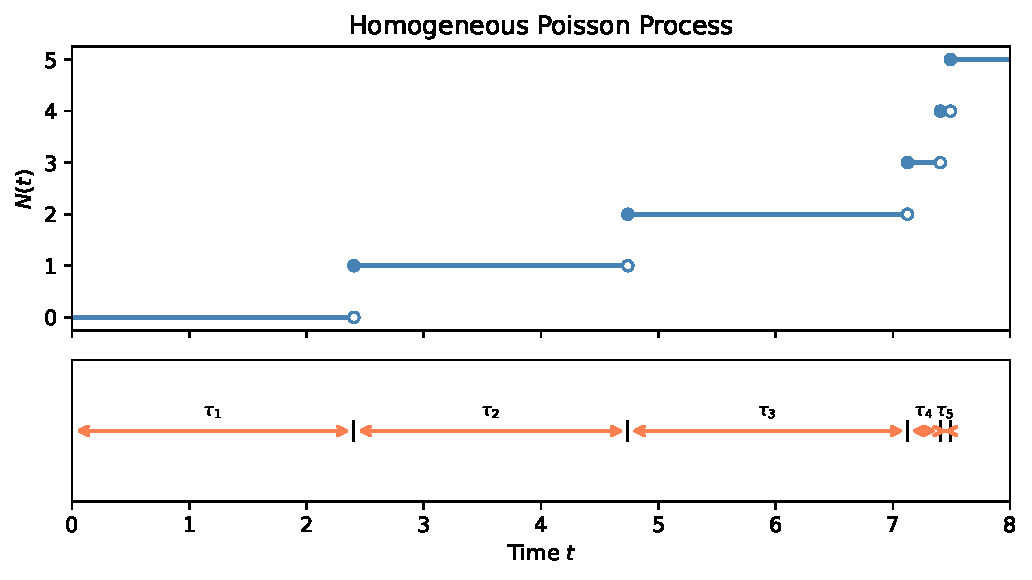
\includegraphics[width=0.78\textwidth]{poisson_process}
\end{center}

\end{frame}

\begin{frame}[fragile]{Python: Homogeneous Poisson Process (Algorithms 73 \& 74)}
\begin{lstlisting}[style=python]
import numpy as np

def simulate_poisson(lam, t_max, rng=None):
    """Algorithm PoiPro: simulate Poisson(lambda) on [0, t_max]."""
    if rng is None:
        rng = np.random.default_rng()
    arrivals = []
    t = -np.log(rng.uniform()) / lam       # first inter-arrival ~ Exp(lam)
    while t <= t_max:
        arrivals.append(t)
        t += -np.log(rng.uniform()) / lam  # next inter-arrival
    return np.array(arrivals)

def simulate_poisson_sorted(lam, t_max, rng=None):
    """Algorithm PoiProSorted: simulate via order-statistics."""
    if rng is None:
        rng = np.random.default_rng()
    K = rng.poisson(lam * t_max)           # total number of arrivals
    arrivals = rng.uniform(0, t_max, size=K)
    return np.sort(arrivals)

# Example: lambda=2, simulate on [0,10]; expected ~20 arrivals
rng = np.random.default_rng(42)
A = simulate_poisson(lam=2.0, t_max=10.0, rng=rng)
print(f"Inter-arrival method: {len(A)} arrivals")  # expect ~20
B = simulate_poisson_sorted(lam=2.0, t_max=10.0, rng=rng)
print(f"Sorted method:        {len(B)} arrivals")
\end{lstlisting}
\end{frame}

% ── 8.2.2 ────────────────────────────────────────────────
\subsection{8.2.2 Non-homogeneous Poisson Process}

\begin{frame}[allowframebreaks]{8.2.2 Non-homogeneous Poisson Process (NHPP)}

A homogeneous Poisson process has the same arrival rate $\lambda$ at all times.
This is inadequate for many real-world systems: call centers have peak hours,
retail stores have rush periods, and network traffic varies throughout the day.
A \textbf{non-homogeneous Poisson process} (NHPP) generalizes this by allowing
the intensity to be a function of time, $\lambda(t)$.

\begin{block}{Definition 8.2.3 -- Non-homogeneous Poisson Process}
A counting process $N(t)$ is a \textbf{non-homogeneous Poisson process} (NHPP)
with \textbf{intensity function} $\lambda(t) \ge 0$ if:
\begin{enumerate}
  \item Numbers of arrivals in disjoint intervals are independent.
  \item The count $N(s, t]$ has a Poisson distribution with mean
        $\int_s^t\lambda(u)\,du$ (integral of lambda from $s$ to $t$).
\end{enumerate}
\end{block}

Here $\lambda(t)$ (lambda of t) is the local arrival rate at time $t$: the
expected number of arrivals in a tiny window $[t, t+dt]$ equals $\lambda(t)\,dt$.
When $\lambda(t) = \lambda$ is constant, the NHPP reduces to the homogeneous case.

\framebreak

\textbf{Thinning Algorithm.}  The main simulation technique for NHPPs is
\textbf{thinning} (also called Lewis-Shedler thinning).  The idea is elegant:
first generate arrivals at the maximum possible rate $\lambda_{\max}$ (an
upper bound on $\lambda(t)$ over the simulation interval), then randomly
\emph{discard} each proposed arrival with probability proportional to how much
the true rate falls short of the maximum.

\begin{block}{Proposition 8.2.4 -- Thinning}
Let $\lambda_{\max} \ge \lambda(t)$ for all $t \in (0, t_{\max})$.  Generate a
homogeneous Poisson process at rate $\lambda_{\max}$ to produce candidate
arrivals.  Retain each candidate arrival at time $A_i$ independently with
probability
\[
  p(A_i) = \frac{\lambda(A_i)}{\lambda_{\max}}.
\]
Here $p(A_i)$ (p of A sub i) is the \textbf{acceptance probability} at time
$A_i$.  The retained (thinned) process is an NHPP with intensity $\lambda(t)$.
\end{block}

Intuitively, we ``oversample'' at the maximum rate and then randomly discard
points with higher probability at times when the true rate is low.  At the
maximum rate time $\lambda(t) = \lambda_{\max}$, every candidate is accepted
($p=1$); at a quiet time where $\lambda(t) = 0.1\,\lambda_{\max}$, only 10\%
are accepted.

\begin{block}{Algorithm 75 -- NH-Poi-thinning($\lambda(t)$)}
\textbf{Require:} $\lambda_{\max} = \max_{t \in [0,t_{\max}]}\lambda(t)$.
\begin{enumerate}
  \item Create empty list $\mathtt{A}$; draw $U \sim \mathcal{U}(0,1)$; set
        $t = -\log(U)/\lambda_{\max}$.
  \item \textbf{While} $t \le t_{\max}$: compute acceptance probability
        $p = \lambda(t)/\lambda_{\max}$; draw $U_1 \sim \mathcal{U}(0,1)$;
        if $U_1 \le p$, accept and append $t$; then draw
        $U_2 \sim \mathcal{U}(0,1)$ and set $t \leftarrow t -
        \log(U_2)/\lambda_{\max}$.
  \item Return $\mathtt{A}$.
\end{enumerate}
\end{block}

\begin{center}
  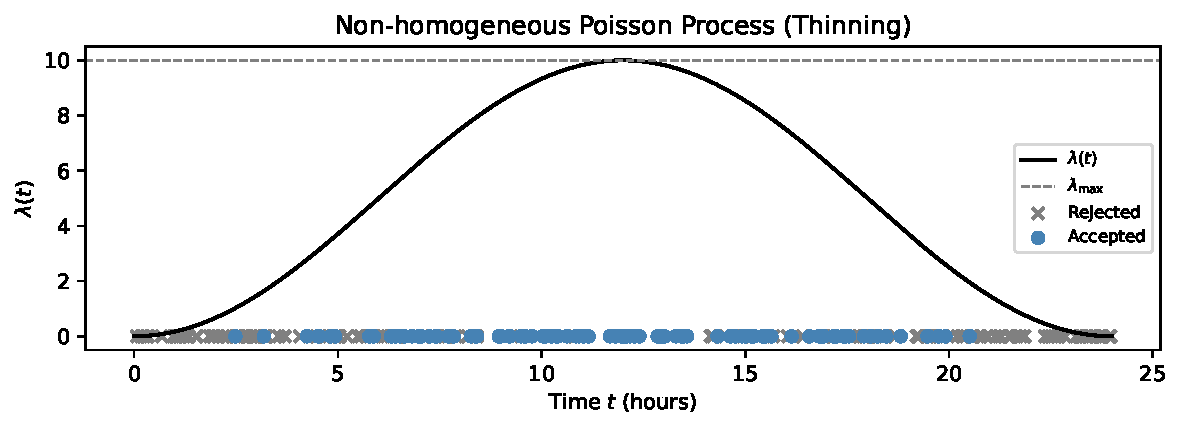
\includegraphics[width=0.68\textwidth]{nhpp_thinning}
\end{center}

\framebreak

\textbf{Inversion Method.}  An alternative approach uses the \emph{integrated
intensity} function $h(t) = \int_0^t \lambda(s)\,ds$ (h of t, the cumulative
intensity up to time $t$).

\begin{block}{Algorithm 76 -- NH-Poi($\lambda(t)$): Inversion Method}
\begin{enumerate}
  \item Sample $K \sim \mathrm{Poi}\!\left(h(t_{\max})\right)$.
  \item Compute the c.d.f.\ $F(s) = h(s)/h(t_{\max})$ and its generalized
        inverse $F^{\leftarrow}$ (the quantile function).
  \item Draw $U_1,\ldots,U_K \overset{\rm iid}{\sim} \mathcal{U}(0,1)$; set
        $A_i = F^{\leftarrow}(U_i)$.
  \item Return sorted values $(A_{(1)},\ldots,A_{(K)})$.
\end{enumerate}
\end{block}

Algorithm 76 requires computing $F^{\leftarrow}$ analytically or numerically,
which is extra work not needed by the thinning algorithm.  The thinning approach
(Algorithm 75) is therefore more widely used in practice.

\begin{exampleblock}{Worked Example: Sinusoidal Call Center}
Suppose $\lambda(t) = 10(0.5 + 0.5\sin(2\pi t/24 - \pi/2))$ models a call
center with a daily cycle (24 hours).  At midnight ($t=0$), $\lambda(0) = 0$:
no calls.  At noon ($t=12$), $\lambda(12) = 10$: peak 10 calls/hour.  The
maximum is $\lambda_{\max} = 10$.  In the thinning algorithm: we propose
arrivals at rate 10, then accept each one at time $t$ with probability
$p(t) = \lambda(t)/10 = 0.5 + 0.5\sin(2\pi t/24 - \pi/2)$.  The expected
total number of calls in a day is $\int_0^{24}\lambda(t)\,dt = 10\cdot 12 = 120$.
\end{exampleblock}

\end{frame}

\begin{frame}[fragile]{Python: NHPP Thinning (Algorithm 75)}
\begin{lstlisting}[style=python]
import numpy as np

def nhpp_thinning(lam_func, lam_max, t_max, rng=None):
    """NH-Poi-thinning: simulate NHPP with intensity lam_func(t).
    lam_func must satisfy lam_func(t) <= lam_max for all t in [0,t_max]."""
    if rng is None:
        rng = np.random.default_rng()
    A = []
    t = -np.log(rng.uniform()) / lam_max   # first candidate ~ Exp(lam_max)
    while t <= t_max:
        p = lam_func(t) / lam_max          # acceptance probability
        if rng.uniform() <= p:             # accept with prob p
            A.append(t)
        t += -np.log(rng.uniform()) / lam_max   # next candidate
    return np.array(A)

# Sinusoidal daily pattern: peaks at noon (t=12), quiet at midnight
# lambda(t) = 10 * (0.5 + 0.5 * sin(2*pi*t/24 - pi/2))
lam_func = lambda t: 10 * (0.5 + 0.5 * np.sin(2*np.pi*t/24 - np.pi/2))
rng = np.random.default_rng(7)
A = nhpp_thinning(lam_func, lam_max=10.0, t_max=24.0, rng=rng)
print(f"Arrivals in one day: {len(A)}")   # expected ~120
print(f"First five arrival times (hours): {np.array(A[:5]).round(2)}")
\end{lstlisting}
\end{frame}

% ── 8.2.3 ────────────────────────────────────────────────
\subsection{8.2.3 Poisson Process on General Spaces}

\begin{frame}[allowframebreaks]{8.2.3 Poisson Process on General Spaces}

So far, arrivals occur on the time axis $[0, t_{\max}]$.  The Poisson process
generalizes naturally to any measurable space $E \subset \R^d$, such as a
two-dimensional spatial region (e.g., locations of customers in a city), or a
product space of time and location.  This generalization is called a
\textbf{Poisson point process}.

\begin{block}{Definition 8.2.6 -- Poisson Point Process on $E \subset \R^d$}
Let $E \subset \mathbb{R}^d$ (R to the power d, meaning $d$-dimensional
Euclidean space) be a region with \textbf{intensity measure} $\Lambda$
(Lambda, capital lambda).  A point process $N$ on $E$ is a \textbf{Poisson
point process} with intensity measure $\Lambda$ if:
\begin{enumerate}
  \item For all disjoint sets $B_1, \ldots, B_n \subset E$, the random
        variables $N(B_1), \ldots, N(B_n)$ are independent.
  \item $N(B) \sim \mathrm{Poi}(\Lambda(B))$ for every measurable $B \subset E$.
\end{enumerate}
Here $N(B)$ denotes the number of points falling inside the region $B$.
\end{block}

Special cases reveal the connections to earlier models:
\begin{itemize}
  \item On $E = [0, t_{\max}]$ with $\Lambda(dt) = \lambda\,dt$ (Lambda equals
        lambda times dt): this is the homogeneous Poisson process.
  \item With $\Lambda(dt) = \lambda(t)\,dt$: the NHPP.
  \item On a rectangle $E \subset \R^2$ with $\Lambda(d\mathbf{x}) =
        \lambda\,d\mathbf{x}$: a spatial Poisson process used in queueing
        network models and wireless communications.
\end{itemize}

\framebreak

When $\Lambda(E) < \infty$ (the total intensity is finite), the total number of
points is a.s.\ finite and the process is easy to simulate.

\begin{block}{Algorithm 77 -- Poisson Process on $E$ with Finite $\Lambda(E)$}
\begin{enumerate}
  \item Generate $T \sim \mathrm{Poi}(\Lambda(E))$.  Here $T$ is the total
        number of points; its expected value is $\Lambda(E)$.
  \item Draw $\xi_1, \ldots, \xi_T$ (xi sub 1 to T) independently from $E$
        with distribution $\Lambda(d\mathbf{x})/\Lambda(E)$ (the normalized
        intensity measure, which is a probability distribution on $E$).
  \item Return the random set $\{\xi_1, \ldots, \xi_T\}$.
\end{enumerate}
\end{block}

When $\Lambda(E) = \infty$ but $E = \bigcup_{j=1}^\infty E_j$ with
$\Lambda(E_j) < \infty$ for each $j$, one simulates independent Poisson
processes on each subregion $E_j$ and superimposes the results.  The
\emph{superposition property} of Poisson processes guarantees the result is
still a Poisson process.

\begin{columns}
  \column{0.50\textwidth}
  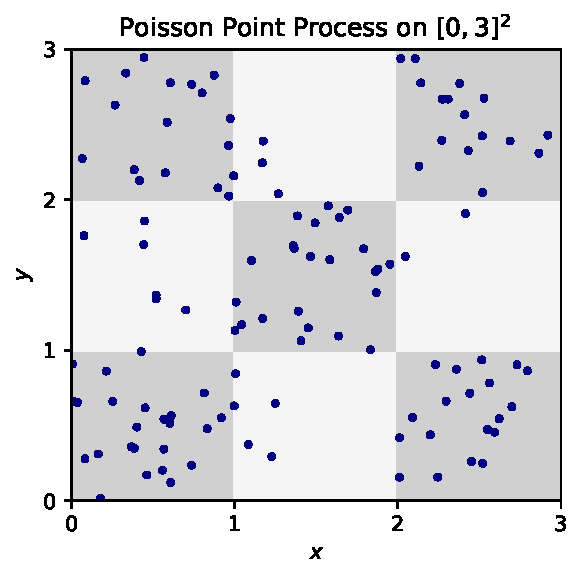
\includegraphics[width=\textwidth]{poisson_2d}
  \column{0.48\textwidth}
  \textbf{Example (Fig.\ 8.3):} Heterogeneous intensity on $[0,3]^2$.
  The domain is partitioned into 9 cells $E_1,\ldots,E_9$.  Grey (shaded)
  cells have intensity $\Lambda = 20$ points per cell; light cells have
  $\Lambda = 5$.  Each cell independently generates a Poisson number of
  uniformly distributed points.  The two simulations (left and right) are
  independent realizations of the same model.
\end{columns}

\end{frame}

% ============================================================
\section{8.3 Birth and Death Processes / Markovian Queues}
% ============================================================

\begin{frame}[allowframebreaks]{8.3 Birth-and-Death Processes and Markovian Queues}

The simplest queueing models have the Markov property: given the current number
of tasks $L(t) = i$ in the system at time $t$, the future behavior of the queue
depends only on $i$ and not on the entire history of arrivals and departures.
These models are called \textbf{birth-and-death (B\&D) processes}.

``Birth'' means an arrival (the queue length increases by 1); ``death'' means a
departure (the queue length decreases by 1).

\begin{block}{Birth-and-Death Process}
A continuous-time Markov process $X(t)$ on state space $\{0, 1, 2, \ldots\}$
is a \textbf{birth-and-death process} with birth rates $(\lambda_i)_{i\ge 0}$
(lambda sub i) and death rates $(\mu_i)_{i\ge 1}$ (mu sub i, with $\mu_0 = 0$)
if, when in state $i$:
\begin{itemize}
  \item A \emph{birth} (jump up to state $i+1$) occurs at rate $\lambda_i$.
  \item A \emph{death} (jump down to state $i-1$) occurs at rate $\mu_i$
        (only possible if $i \ge 1$).
  \item The time until the next event is $\tau \sim \mathrm{Exp}(\lambda_i +
        \mu_i)$ (exponential with rate equal to the total event rate).
  \item Given that an event occurs, it is a birth with probability
        $\lambda_i/(\lambda_i + \mu_i)$ and a death otherwise.
\end{itemize}
\end{block}

The simulation algorithm proceeds event by event: at each step, draw the sojourn
time from the appropriate exponential distribution, then decide birth or death by
a Bernoulli trial.

\framebreak

\begin{block}{Kendall Notation for Queues: A/S/c}
Standard queueing systems are described by three symbols separated by slashes:
\begin{itemize}
  \item \textbf{A} = arrival (inter-arrival time) distribution: \textbf{M} =
        Markovian (i.e., exponential, memoryless), \textbf{G} = general,
        \textbf{GI} = i.i.d.\ general, \textbf{D} = deterministic.
  \item \textbf{S} = service time distribution: same symbols.
  \item \textbf{c} = number of servers; $c = \infty$ means every task
        immediately starts service (no waiting possible).
\end{itemize}
\end{block}

The \textbf{M/M/1 queue} is the fundamental single-server queue: Poisson
arrivals at rate $\lambda$ and exponential service times with rate $\mu$ (so
mean service time $= 1/\mu$).  It is a B\&D process with $\lambda_i = \lambda$
and $\mu_i = \mu$ for all valid $i$.

Stability requires the arrival rate to be strictly less than the service rate.
The \textbf{traffic intensity} $\rho = \lambda/\mu$ (rho, Greek letter
``rho'') captures this: $\rho < 1$ for stability, $\rho \ge 1$ for instability.

\begin{block}{M/M/1 Steady-State Distribution and Mean Queue Length}
When $\rho < 1$, the stationary distribution of the queue length $L^*$ (L-star,
the queue length in steady state) is \emph{geometric}:
\[
  \pi_i = \Prob(L^* = i) = (1-\rho)\,\rho^i, \qquad i = 0, 1, 2, \ldots
\]
The steady-state mean number of tasks in the system is:
\[
  \bar{l} = \E[L^*] = \sum_{i=0}^\infty i\,(1-\rho)\rho^i = \frac{\rho}{1-\rho}
          = \frac{\lambda}{\mu-\lambda}.
\]
Here $\bar{l}$ (l-bar) denotes the long-run average queue length, and
$\pi_i$ (pi sub i) is the probability of being in state $i$ in steady state.
When $\rho \ge 1$, the queue is unstable: $L(t) \to \infty$ almost surely.
\end{block}

\framebreak

\begin{exampleblock}{Worked Example: M/M/1 Queue Length}
Take $\lambda = 0.5$ arrivals per unit time, $\mu = 1$ service per unit time.
Then $\rho = 0.5/1 = 0.5$.  The mean queue length is $\bar{l} = 0.5/(1-0.5) = 1$.
The probability of an empty system is $\pi_0 = 1 - \rho = 0.5$, i.e., the
server is idle 50\% of the time.

Now take $\lambda = 8/9$, $\mu = 1$, so $\rho = 8/9 \approx 0.889$.  Then
$\bar{l} = (8/9)/(1/9) = 8$.  The system has 8 customers on average even though
it is stable.  Going from $\rho = 0.5$ to $\rho = 0.889$ increased the mean
queue length 8-fold!  This illustrates how sensitive queueing systems are to the
traffic intensity near 1.
\end{exampleblock}

To estimate $\bar{l}$ from a simulation run on $[0, t_{\max}]$, we compute the
time-weighted average of the queue length.  If the simulated jump times are
$0 = a_0 < a_1 < \cdots < a_k \le t_{\max}$ and $y_j = L(a_j)$ is the queue
length in the interval $[a_j, a_{j+1})$, then:
\[
  \hat{l}(t_{\max}) = \frac{1}{t_{\max}}\int_0^{t_{\max}} L(s)\,ds
                    = \frac{1}{t_{\max}}\sum_{j=0}^{k} y_j\,(a_{j+1}-a_j).
\]

\begin{columns}
  \column{0.52\textwidth}
  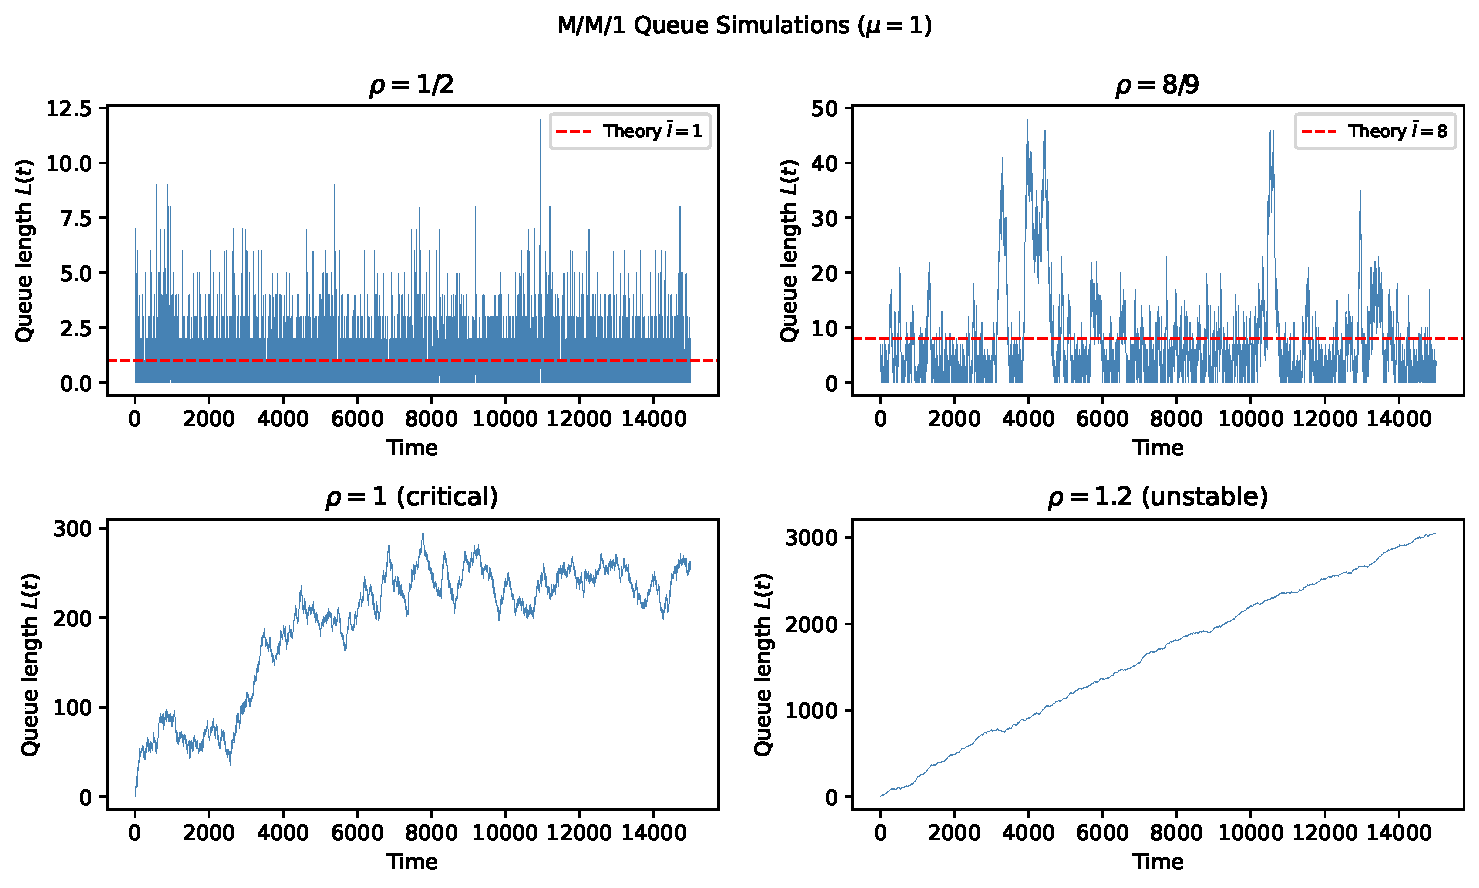
\includegraphics[width=\textwidth]{mm1_simulations}
  \column{0.46\textwidth}
  \textbf{Fig.\ 8.4:} Simulations of $L(t)$ for $\mu=1$ and four values of
  $\lambda$:
  \textbf{(a)} $\rho=0.5$: stable, $\bar{l}=1$, estimate $\hat{l}=0.98$.
  \textbf{(b)} $\rho=8/9$: stable, $\bar{l}=8$, but estimate $\hat{l}=6.67$
  (run too short).
  \textbf{(c)} $\rho=1$: critical, mean diverges.
  \textbf{(d)} $\rho=1.2$: unstable, $L(t)\to\infty$.
\end{columns}

\end{frame}

\begin{frame}[fragile]{Python: Birth-and-Death / M/M/1 Simulation (Algorithm 78)}
\begin{lstlisting}[style=python]
import numpy as np

def simulate_bd(lam_func, mu_func, t_max, y0=0, rng=None):
    """Algorithm 78: Simulate a birth-and-death process on [0, t_max].
    lam_func(i) = birth rate from state i, mu_func(i) = death rate."""
    if rng is None:
        rng = np.random.default_rng()
    t, y = 0.0, y0
    JS = [(0.0, y0)]  # list of (time, state) pairs
    while t < t_max:
        lam_i = lam_func(y)
        mu_i  = mu_func(y)
        rate  = lam_i + mu_i
        if rate == 0:
            break
        t += rng.exponential(1.0 / rate)   # time until next event
        if t >= t_max:
            break
        u = rng.uniform()
        y = y + 1 if u < lam_i / rate else max(y - 1, 0)  # birth or death
        JS.append((t, y))
    JS.append((t_max, y))
    times  = np.array([e[0] for e in JS])
    states = np.array([e[1] for e in JS])
    l_hat  = np.sum(states[:-1] * np.diff(times)) / t_max
    return l_hat, JS

# M/M/1: lambda=0.5, mu=1.0, theoretical mean = rho/(1-rho) = 1.0
rng = np.random.default_rng(0)
l_hat, _ = simulate_bd(lambda i: 0.5, lambda i: 1.0 if i > 0 else 0.0,
                        t_max=1e4, rng=rng)
print(f"Estimated mean queue length: {l_hat:.4f}  (theory: 1.0000)")
\end{lstlisting}
\end{frame}

% ============================================================
\section{8.4 Basic Concepts of Queueing Theory}
% ============================================================

\begin{frame}[allowframebreaks]{8.4 Basic Concepts of Queueing Theory}

We now set up the general notation for single- and multi-server queues and
introduce the key performance measures.  Consider a queue with tasks (customers)
arriving one by one.  For the $i$-th task:
\begin{itemize}
  \item $A_i$ = arrival time (when the task joins the system).
  \item $S_i$ = service time (how long the task takes to process, once started).
  \item $W_i$ = waiting time (time spent in the queue before service starts).
  \item $D_i = A_i + W_i + S_i$ = departure time (when the task leaves).
  \item Sojourn time (total time in system) $= W_i + S_i$.
\end{itemize}
The process $L(t)$ = number of tasks in the system at time $t$ (including those
currently being served).

\begin{columns}
  \column{0.55\textwidth}
  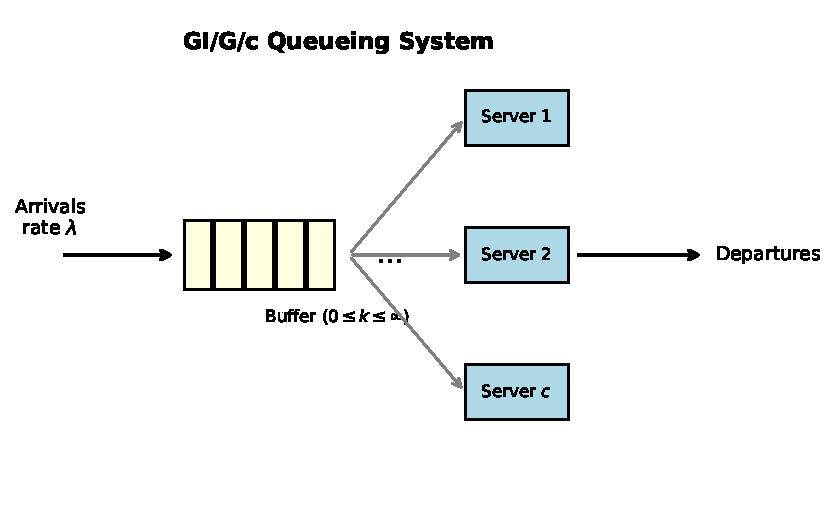
\includegraphics[width=\textwidth]{queue_diagram}
  \column{0.43\textwidth}
  The two standard configurations are: (left) one shared queue feeding into
  multiple servers, and (right) a separate queue per server.  In the shared-queue
  model, each arriving task joins a single waiting line and is served by the next
  available server -- this is the ``M/M/c'' or ``GI/G/c'' model.
\end{columns}

\framebreak

\begin{block}{Traffic Intensity $\varrho$}
The \textbf{traffic intensity} (also called the \textbf{load} or
\textbf{utilization}) is
\[
  \varrho = \frac{\E[S_1]}{\E[\tau_1]} = \lambda \E[S_1],
\]
where $\E[S_1]$ (E of S sub 1) is the mean service time, $\E[\tau_1]$ is the
mean inter-arrival time, and $\lambda = 1/\E[\tau_1]$ (lambda) is the arrival
rate.  The symbol $\varrho$ (varrho, a variant of ``rho'') measures how much
work arrives per unit time relative to the service capacity.

For a $c$-server system, stability requires $\varrho < c$; with one server
($c=1$), stability requires $\varrho < 1$.
\end{block}

\begin{block}{Little's Law}
Under mild conditions, for \emph{any} stable queueing system, regardless of
arrival or service distributions:
\[
  \bar{l} = \lambda\,\bar{w},
\]
where $\bar{l}$ (l-bar) is the steady-state mean number of tasks in the system,
$\lambda$ (lambda) is the arrival rate, and $\bar{w}$ (w-bar) is the steady-state
mean \emph{sojourn time} (total time from arrival to departure).
\end{block}

Little's Law is remarkable because it holds universally -- no matter how complex
the queueing system.  It connects the three most important performance measures:
occupancy, throughput, and latency.

\begin{columns}
  \column{0.52\textwidth}
  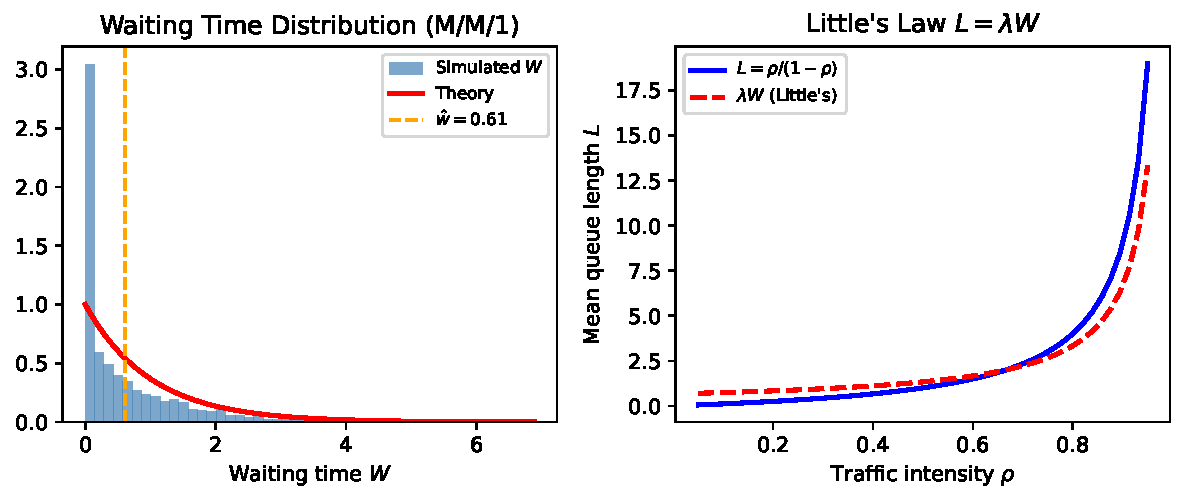
\includegraphics[width=\textwidth]{littles_law}
  \column{0.46\textwidth}
  \textbf{Application to M/M/1:}
  We know $\bar{l} = \rho/(1-\rho)$.  Applying Little's Law:
  \[
    \bar{w} = \frac{\bar{l}}{\lambda} = \frac{1}{\mu - \lambda}.
  \]
  With $\lambda=0.5$, $\mu=1$: $\bar{l}=1$ task average, and
  $\bar{w}=2$ time units sojourn per task.
\end{columns}

\framebreak

\begin{block}{Lindley Recursion for GI/G/1 -- Equation (8.4.1)}
Under the First Come First Served (FCFS) discipline with one server, the waiting
times satisfy a simple recursion.  Starting with $W_1 = 0$ (first task finds the
system empty):
\[
  W_{i+1} = (W_i + S_i - \tau_{i+1})_+, \qquad i = 1, 2, \ldots
\]
Here $(x)_+ = \max(x, 0)$ (the positive part of $x$).

Reading this formula: when the $(i+1)$-th task arrives, the server has been
busy for $W_i + S_i$ total time since task $i$ arrived.  If another $\tau_{i+1}$
time units have elapsed since task $i$'s arrival (the inter-arrival time), then
the remaining work is $W_i + S_i - \tau_{i+1}$.  If this is negative, the server
was idle before task $i+1$ arrived, so $W_{i+1} = 0$.
\end{block}

\begin{alertblock}{How to Read the Lindley Recursion}
Think of $W_i + S_i$ as the ``workload'' the server inherits from task $i$: it
must finish task $i$ before starting $i+1$.  Subtracting $\tau_{i+1}$ gives the
remaining workload when task $i+1$ arrives.  If positive, task $i+1$ waits; if
negative, it finds the server idle.  This recursion is valid for \emph{any}
sample path, not just in expectation.
\end{alertblock}

\begin{block}{Pollaczek-Khinchin (PK) Formula for M/G/1}
When arrivals are Poisson at rate $\lambda$ and service times have general
distribution with $\E[S_1] = 1/\mu$ and second moment $\E[S_1^2] < \infty$:
\[
  \tilde{w} = \frac{\lambda \E[S_1^2]}{2(1 - \lambda\E[S_1])}.
\]
Here $\tilde{w}$ (w-tilde) is the steady-state mean waiting time in queue.
$\E[S_1^2]$ captures the variability of service times: more variable service
leads to longer waiting even with the same average service rate.  For
exponential service ($S \sim \mathrm{Exp}(\mu)$, $\E[S^2] = 2/\mu^2$):
$\tilde{w} = \rho/(\mu(1-\rho))$.
\end{block}

\framebreak

\begin{block}{M/G/$\infty$ System: Infinite Servers, No Waiting}
In an infinite-server system, each arriving task immediately starts service; no
task ever waits.  With Poisson arrivals (rate $\lambda$), i.i.d.\ service times
$S \sim G$ with mean $\E[S] = 1/\mu$, and load $\varrho = \lambda/\mu$:
\[
  \Prob(L^* = k) = \frac{\varrho^k}{k!}e^{-\varrho}, \qquad k = 0, 1, \ldots
\]
The steady-state distribution of the number of tasks present is Poisson with
mean $\varrho$.  Crucially, this holds for \emph{any} service distribution $G$
-- only the mean service time $\E[S]$ matters.
\end{block}

\begin{exampleblock}{Worked Example: GI/G/1 Waiting Times (Table 8.1)}
Five tasks with inter-arrival times $\tau_i$ and service times $S_i$:\\[0.3em]
$(\tau_1,S_1)=(1.0,\,2.5)$, $(\tau_2,S_2)=(1.5,\,2.5)$,
$(\tau_3,S_3)=(4.5,\,0.5)$, $(\tau_4,S_4)=(1.0,\,5)$, $(\tau_5,S_5)=(1.0,\,1)$.\\[0.3em]
Arrival times: $A_1=1$, $A_2=2.5$, $A_3=7$, $A_4=8$, $A_5=9$.\\
Applying the Lindley recursion with $W_1=0$:
\begin{align*}
  W_2 &= (W_1+S_1-\tau_2)_+ = (0+2.5-1.5)_+ = 1.0\\
  W_3 &= (W_2+S_2-\tau_3)_+ = (1+2.5-4.5)_+ = 0.0\\
  W_4 &= (W_3+S_3-\tau_4)_+ = (0+0.5-1.0)_+ = 0.0\\
  W_5 &= (W_4+S_4-\tau_5)_+ = (0+5-1.0)_+ = 4.0
\end{align*}
Departure times: $D_i = A_i+W_i+S_i$: $D_1=3.5$, $D_2=6$, $D_3=7.5$,
$D_4=13$, $D_5=14$.
\end{exampleblock}

\end{frame}

% ============================================================
\section{8.5 Discrete-Event Simulations}
% ============================================================

\begin{frame}[allowframebreaks]{8.5 Discrete-Event Simulations -- The General Framework}

Many processes change state only at specific \emph{event times} --- arrivals,
departures, failures, repairs, slot boundaries.  Between consecutive events,
the system state remains constant.  A \textbf{discrete-event simulation (DES)}
exploits this structure by advancing the simulation clock directly to the next
event rather than stepping through time in small fixed increments (which would
be very wasteful when events are infrequent).

\begin{block}{Core Components of a Discrete-Event Simulation}
\begin{enumerate}
  \item \textbf{Simulation clock} $t$: the current simulated time.
  \item \textbf{Event list} (EL): a sorted list of pending events, each tagged
        with its scheduled time and type (arrival, departure, failure, etc.).
        The simulation always processes the event with the smallest time first.
  \item \textbf{State variables}: e.g., $n$ = current number of tasks in the
        system, queue contents, server status (busy/idle).
  \item \textbf{Output list} JS: records $(t(i), n(i))$ pairs after each event
        for post-processing and estimation.
\end{enumerate}
\end{block}

The DES approach is far more efficient than time-stepping because it skips all
the ``idle'' time between events.  If events are rare (e.g., one per hour), the
time-stepping approach would waste millions of steps during idle periods.

\framebreak

\begin{block}{Example 8.5.1 -- The On-Off Process}
The \textbf{on-off process} $K(t)$ takes values in $\{0, 1\}$ (off or on) and
alternates between state 1 (\emph{on}, e.g., a server is active or a link is
transmitting) and state 0 (\emph{off}, idle).  \emph{On}-time durations
$T_1^{\mathrm{on}}, T_2^{\mathrm{on}}, \ldots$ are i.i.d.\ with distribution
$F_{\mathrm{on}}$; \emph{off}-time durations are i.i.d.\ with distribution
$F_{\mathrm{off}}$.

The steady-state probability of being \emph{on} is:
\[
  p = \frac{\E T^{\mathrm{on}}}{\E T^{\mathrm{on}} + \E T^{\mathrm{off}}},
\]
a consequence of the renewal reward theorem.  This is simply the fraction of
time in the on-state, equal to the mean on-time divided by the mean cycle length.

To estimate $p$ from simulation, compute the time average:
\[
  \hat{p}(t_{\max}) = \frac{1}{t_{\max}}\int_0^{t_{\max}} K(s)\,ds.
\]
This is the fraction of time the process was in state 1 during the simulation.
\end{block}

\begin{center}
  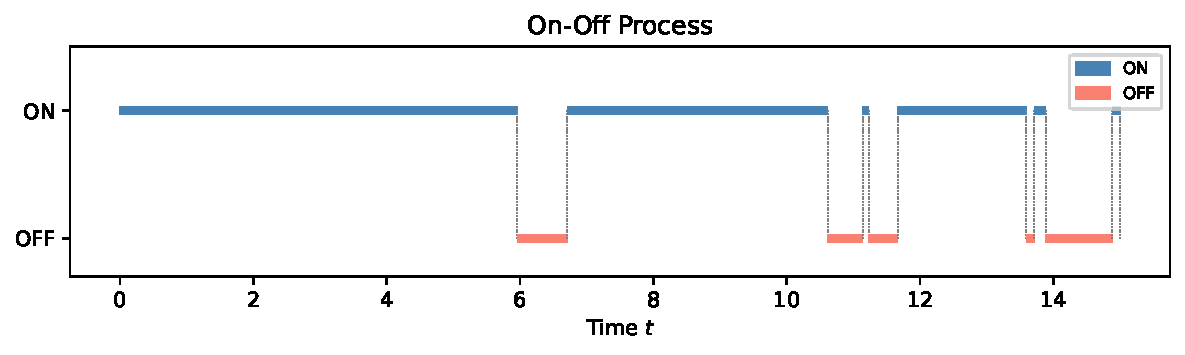
\includegraphics[width=0.76\textwidth]{onoff_process}
\end{center}

\framebreak

\begin{block}{Example 8.5.2 -- Repairman Problem (Algorithm 79)}
A system has $N$ elements (machines) and $M$ repairmen.  Each working element
fails after a random failure time $\tau^f \sim F$; once failed, it waits for a
repairman, then is repaired in time $\tau^r \sim G$.  The state $k(t)$ is the
number of \emph{working} elements at time $t$.

The DES processes two event types:
\begin{itemize}
  \item \textbf{Failure event}: element fails.  Working count decreases by 1.
        If a repairman is free ($s < M$), assign it immediately and schedule
        a repair completion; otherwise add the element to the repair queue.
  \item \textbf{Repair\_Completion event}: a repair finishes.  Working count
        increases by 1.  If elements are waiting, assign the freed repairman
        to the next one and schedule its completion.
\end{itemize}
\end{block}

The time-averaged estimators of interest are:
\[
  \hat{l} = \frac{1}{t}\int_0^t L(s)\,ds \;\text{(mean working)}, \quad
  \hat{m} = N - \hat{l} - \hat{w} \;\text{(mean under repair)},
\]
where $\hat{w}$ is the mean number waiting for repair.  Figure 8.8 illustrates
this for $N=5$ elements and $M=1$ repairman.

\end{frame}

\begin{frame}[fragile]{Python: On-Off Discrete-Event Simulation}
\begin{lstlisting}[style=python]
import numpy as np

def simulate_onoff(F_on, F_off, t_max, rng=None):
    """Discrete-event simulation of on-off process.
    F_on / F_off: callables(rng) returning one sample."""
    if rng is None:
        rng = np.random.default_rng()
    t = 0.0; state = 1   # start in ON state
    integral = 0.0        # accumulate integral of K(t)
    while t < t_max:
        duration = F_on(rng) if state == 1 else F_off(rng)
        new_t = min(t + duration, t_max)
        integral += state * (new_t - t)  # K(s)=state on [t, new_t]
        t = new_t
        if t < t_max:
            state = 1 - state            # flip state
    return integral / t_max              # time-averaged estimator p_hat

rng = np.random.default_rng(5)
# Exponential on/off: E[T^on]=3, E[T^off]=1, theory p = 3/4 = 0.75
p_hat = simulate_onoff(
    F_on  = lambda r: r.exponential(3.0),
    F_off = lambda r: r.exponential(1.0),
    t_max = 50000, rng=rng)
print(f"p_hat = {p_hat:.5f}  (theory = 0.75000)")
\end{lstlisting}
\end{frame}

\subsection{8.5.1 GI/G/1 Queue Simulation}

\begin{frame}[allowframebreaks]{8.5.1 GI/G/1 Queue Simulation (Algorithm 81)}

For a GI/G/1 queue, we can estimate the steady-state mean waiting time
$\tilde{w}$ without simulating the full continuous-time process $L(t)$: we
simply iterate the Lindley recursion to generate $W_1, W_2, \ldots$ and compute
their sample mean.  To also estimate $\bar{l}$ (mean tasks in system), we need
the full discrete-event simulation.

\begin{block}{Algorithm 81 -- Discrete-Event Simulation of GI/G/1}
The state consists of two quantities: $t_A$ (time of next scheduled arrival) and
$t_D$ (time of next scheduled departure; set to $\emptyset$ when server is idle).

\begin{enumerate}
  \item Initialize: generate $\tau \sim F$; set $t_A = \tau$;
        set EL $= [t_A, \emptyset]$; create JS $= [[0,0]]$.
  \item \textbf{While} $t_A < t_{\max}$: examine EL.
    \begin{itemize}
      \item \textbf{Case EL}$=[t_A, \emptyset]$ (server idle): $n := 1$;
            generate $S \sim G$, set $t_D = t_A + S$; generate $\tau \sim F$,
            $t_A := t_A + \tau$; update EL$=[t_A, t_D]$.
      \item \textbf{Case} $t_A < t_D$ (arrival before departure): $n := n+1$;
            record; generate $\tau \sim F$, $t_A := t_A + \tau$.
      \item \textbf{Case} $t_A \ge t_D$ (departure first): $n := n-1$;
            if $n > 0$: generate $S \sim G$, $t_D := t_D + S$; else
            EL$=[t_A, \emptyset]$.
    \end{itemize}
\end{enumerate}
Here $F$ is the inter-arrival distribution and $G$ is the service distribution.
\end{block}

\begin{center}
  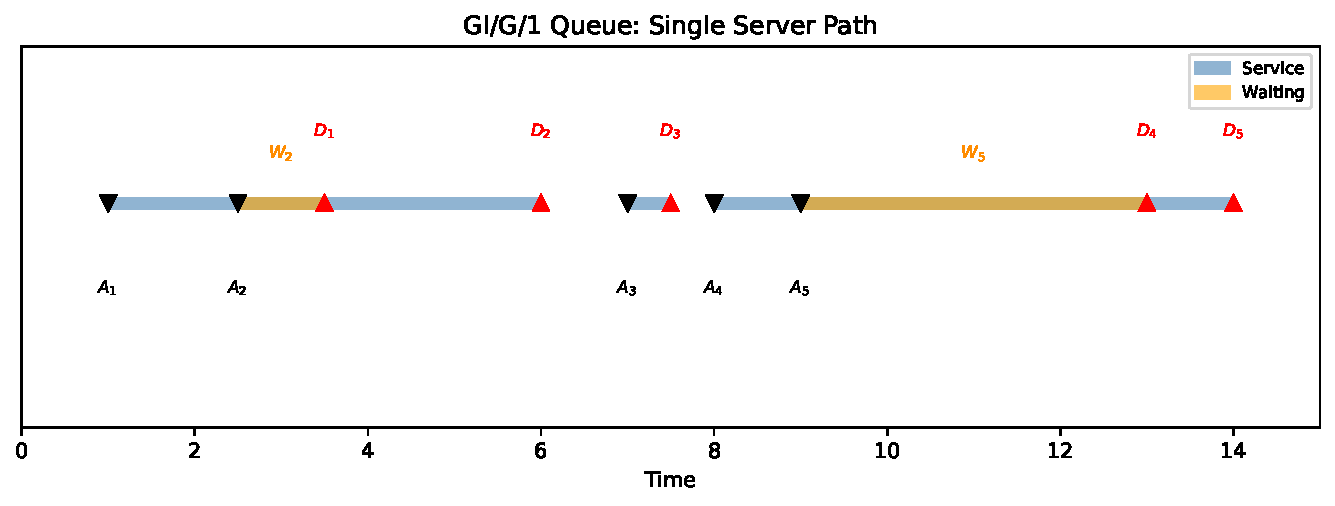
\includegraphics[width=0.76\textwidth]{gig1_path}
\end{center}

\framebreak

Figure 8.9 from the book shows an example path for 5 tasks: arrivals (black
marks), service intervals (blue), waiting intervals (orange), and departures
(red).  The queue length $L(s)$ jumps up at each arrival and down at each
departure.

\begin{block}{GI/G/c Queue: Workload Vector Recursion (Equation 8.5.2)}
For a \textbf{GI/G/c queue} ($c$ servers), we maintain a sorted vector of server
workloads $\mathbf{V}_i = (V_{i,1} \le V_{i,2} \le \cdots \le V_{i,c})$ just
before the $i$-th task arrives.  Here $V_{i,j}$ (V sub i comma j) is the
remaining work at server $j$ when task $i$ arrives.

The waiting time of the $i$-th task is $W_i = V_{i,1}$ (the minimum workload --
it goes to the least-loaded server).  After assignment, the workload vector updates:
\[
  \mathbf{V}_{i+1} = \mathrm{sort}\!\left((V_{i,1} + S_i - \tau_{i+1})_+,\;
                     (V_{i,2} - \tau_{i+1})_+,\; \ldots,\;
                     (V_{i,c} - \tau_{i+1})_+\right).
\]
All workloads decrease by $\tau_{i+1}$ (time passes between arrivals), and task
$i$ adds $S_i$ to the minimum workload.  The sorting step re-orders the workloads.
\end{block}

For $c=1$ this reduces exactly to the Lindley recursion.  If $\varrho =
\E[S]/\E[\tau] < c$, the sequence $\mathbf{V}_i$ has a limiting distribution and:
\[
  \tilde{w} = \lim_{k\to\infty}\frac{1}{k}\sum_{i=1}^k V_{i,1} \quad \text{(a.s.)}.
\]

\end{frame}

\begin{frame}[fragile]{Python: GI/G/1 Waiting Times via Lindley Recursion}
\begin{lstlisting}[style=python]
import numpy as np

def gig1_waiting_times(n_tasks, F_interarr, G_service, rng=None):
    """Lindley recursion: generate waiting times W_1,...,W_n for GI/G/1."""
    if rng is None:
        rng = np.random.default_rng()
    tau = F_interarr(n_tasks, rng)   # inter-arrival times
    S   = G_service(n_tasks, rng)    # service times
    W   = np.zeros(n_tasks)
    for i in range(1, n_tasks):
        W[i] = max(W[i-1] + S[i-1] - tau[i], 0.0)
    return W

rng = np.random.default_rng(0)
# M/G/1: Exp(0.5) inter-arrivals, Exp(1) service
# PK formula: tilde_w = lambda*E[S^2]/(2*(1-lambda*E[S]))
# = 0.5 * 2 / (2 * 0.5) = 1.0
W = gig1_waiting_times(
    n_tasks    = 100000,
    F_interarr = lambda n, r: r.exponential(2.0, n),  # mean=2 = 1/lambda
    G_service  = lambda n, r: r.exponential(1.0, n),  # mean=1 = 1/mu
    rng        = rng)
print(f"Estimated mean waiting time: {np.mean(W):.4f}  (PK theory: 1.0000)")

# M/D/1: deterministic service S=1; PK: tilde_w = 0.5*1/(2*(1-0.5)) = 0.5
W_det = gig1_waiting_times(
    n_tasks    = 100000,
    F_interarr = lambda n, r: r.exponential(2.0, n),
    G_service  = lambda n, r: np.ones(n),             # deterministic S=1
    rng        = rng)
print(f"M/D/1 mean waiting time:     {np.mean(W_det):.4f}  (PK theory: 0.5000)")
\end{lstlisting}
\end{frame}

% ============================================================
\section{8.6 Slotted ALOHA}
% ============================================================

\begin{frame}[allowframebreaks]{8.6 Slotted ALOHA and Random Access Protocols}

\textbf{Slotted ALOHA} is a canonical model of a shared wireless communication
channel.  It was proposed in the 1970s as a simple decentralized protocol where
multiple users share a single channel without coordination.  Time is divided into
fixed-length slots.  Each slot, one or more users may attempt to transmit a packet.
If exactly one user transmits, the packet gets through (success).  If two or more
transmit simultaneously, a \emph{collision} occurs and all packets must be
retransmitted later.

The three main retransmission strategies are:
\begin{itemize}
  \item \textbf{Slotted ALOHA}: after any collision, retransmit in the next slot
        with a fixed probability $h$ (h, the retransmission probability,
        $0 < h < 1$).
  \item \textbf{Exponential Back-off}: retransmit with probability $2^{-i}$ after
        $i$ unsuccessful attempts.  This reduces collisions over time.
  \item \textbf{Ethernet (Finite Exponential Back-off)}: exponential back-off up
        to a maximum of $K$ attempts, after which the packet is discarded.
\end{itemize}

\framebreak

\begin{block}{Slotted ALOHA System Model}
Let $X_n$ (X sub n) be the number of packets \emph{waiting} at the beginning of
slot $n$.  New arrivals in slot $n$ follow $A_n \sim \mathrm{Poi}(\lambda)$
(Poisson with rate $\lambda$, lambda), i.i.d.\ across slots.  Each of the $X_n$
waiting packets independently attempts retransmission with probability $h$, so
the number of retransmission attempts $Y_n \sim \mathrm{Bin}(X_n, h)$
(Binomial with parameters $X_n$ and $h$).  The total number of transmission
attempts in slot $n$ is $Z_n = A_n + Y_n$ (Z sub n equals new arrivals plus
retransmission attempts).

The queue evolves as:
\[
  X_{n+1} = X_n + A_n - \mathbf{1}(Z_n = 1), \qquad n = 0, 1, \ldots
\]
The indicator $\mathbf{1}(Z_n = 1)$ (1 if $Z_n=1$, else 0) equals 1 only when
exactly one packet is transmitted (a success), which removes one packet from the
queue.  If $Z_n = 0$ (no transmissions) or $Z_n \ge 2$ (collision), no packet
is removed.
\end{block}

\begin{block}{Success Probability and Conditional Drift}
Given $X_n = k$ waiting packets, the success probability is:
\[
  \Prob(Z_n=1 \mid X_n=k)
  = e^{-\lambda}\cdot kh(1-h)^{k-1} + \lambda e^{-\lambda}(1-h)^k.
\]
The \textbf{conditional drift} (expected change in queue length per slot) is:
\[
  \E[X_{n+1} - X_n \mid X_n = k]
  = \lambda - e^{-\lambda}\bigl(kh(1-h)^{k-1} + \lambda(1-h)^k\bigr).
\]
As $k \to \infty$, both terms $kh(1-h)^{k-1} \to 0$ and $(1-h)^k \to 0$, so
the drift converges to $\lambda > 0$.  This is the key instability result.
\end{block}

\framebreak

\begin{alertblock}{Key Insight: Slotted ALOHA Is Inherently Unstable}
For any fixed retransmission probability $h$ and any arrival rate $\lambda > 0$,
the Markov chain $(X_n)$ is \textbf{transient}: the queue length drifts to
infinity with probability 1.  For large queues, so many packets attempt
retransmission simultaneously that collisions become overwhelming, reducing the
effective throughput below $\lambda$.  The system eventually ``jams''.

The theoretical channel capacity of Slotted ALOHA is $1/e \approx 0.368$
packets per slot (the maximum achievable throughput), but even for arrival rates
well below this capacity, the queue grows without bound under a fixed
retransmission probability $h$.
\end{alertblock}

\begin{columns}
  \column{0.52\textwidth}
  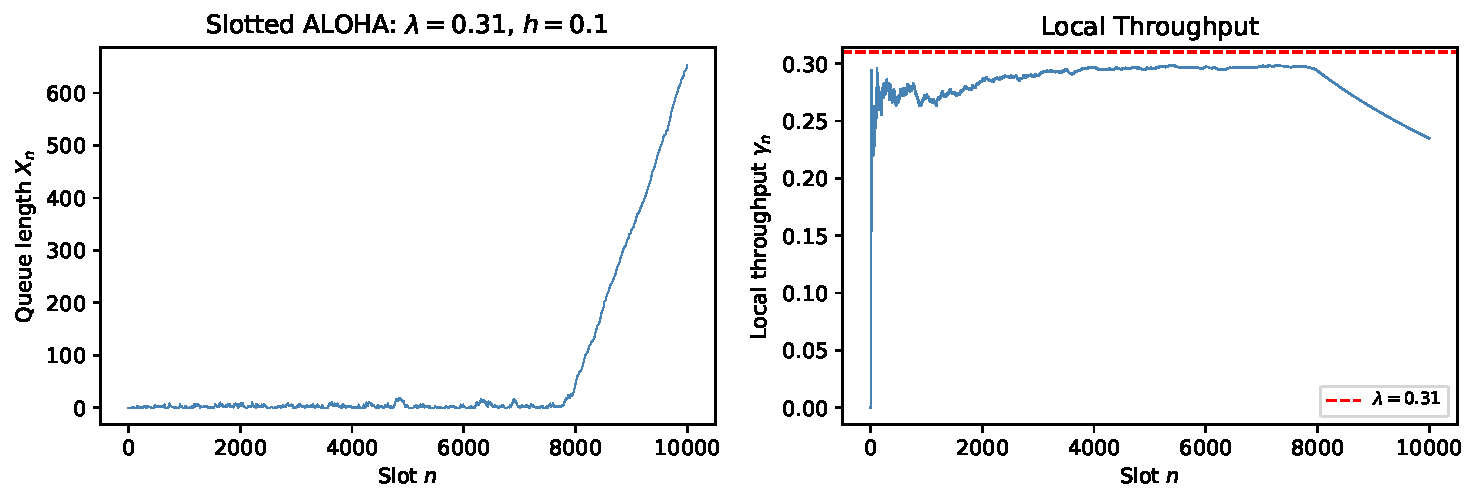
\includegraphics[width=\textwidth]{slotted_aloha}
  \column{0.46\textwidth}
  \textbf{Fig.\ 8.11:} Slotted ALOHA with $\lambda=0.31$, $h=0.1$.\\
  \textbf{(a)} Queue length $X_n$: stable-looking for $\sim$5000 slots, then
  grows linearly.\\
  \textbf{(b)} Local throughput $\gamma_n = N_n^s/n$ (ratio of successes to
  slots): initially $\approx 0.31$, then collapses as collisions dominate.
  This is a classic example of a ``metastable'' system.
\end{columns}

\end{frame}

\begin{frame}[fragile]{Python: Slotted ALOHA Simulation}
\begin{lstlisting}[style=python]
import numpy as np

def simulate_aloha(lam, h, n_slots, X0=0, rng=None):
    """Simulate Slotted ALOHA with Poisson(lam) arrivals per slot.
    h = retransmission probability. Returns queue lengths and throughputs."""
    if rng is None:
        rng = np.random.default_rng()
    X = X0
    Xs = [X0]; successes = 0; throughputs = [0.0]
    for n in range(1, n_slots + 1):
        A = rng.poisson(lam)                       # new arrivals
        Y = rng.binomial(X, h) if X > 0 else 0    # retransmission attempts
        Z = A + Y                                  # total transmissions
        success = int(Z == 1)                      # 1 iff exactly one
        successes += success
        X = max(X + A - success, 0)
        Xs.append(X)
        throughputs.append(successes / n)
    return np.array(Xs), np.array(throughputs)

# lambda=0.31 is well below channel capacity 1/e~0.368, yet system is unstable
rng = np.random.default_rng(11)
Xs, gammas = simulate_aloha(lam=0.31, h=0.1, n_slots=10000, rng=rng)
print(f"Final queue length: {Xs[-1]}")
print(f"Final throughput:   {gammas[-1]:.4f}  (initial rate was ~0.31)")
\end{lstlisting}
\end{frame}

% ============================================================
\section{8.7 Ergodically Stable Processes}
% ============================================================

\begin{frame}[allowframebreaks]{8.7 Ergodically Stable Processes}

To justify using a time average from a single simulation run as an estimator for
a steady-state quantity, we need the concept of \emph{ergodic stability}.  We
build up to it step by step: stationarity, ergodicity, then ergodic stability.

\begin{block}{Stationary Processes}
A stochastic process $(X^*(t))_{t\ge 0}$ (X-star of t) is \textbf{stationary}
if for all $d \ge 1$ and all time shifts $0 < h_1 < \cdots < h_d$, the joint
distribution of $(X^*(t+h_1), \ldots, X^*(t+h_d))$ does not depend on $t$.

Consequences:
\begin{itemize}
  \item The marginal distribution $\Prob(X^*(t) \in B)$ is the same for all
        $t$; so $\E[X^*(t)]$ and $\Var[X^*(t)]$ are constant over time.
  \item The covariance function $R(h) = \mathrm{Cov}(X^*(t), X^*(t+h))$ (R of
        h, the covariance between values at times $t$ and $t+h$) depends only
        on the \emph{lag} $h$, not on $t$.
\end{itemize}
\end{block}

\begin{block}{Ergodic Processes (Equation 8.7.2)}
A stationary process $(X^*(t))$ is \textbf{ergodic} if for any measurable
function $g$ with $\E[|g(X^*(h_1),\ldots,X^*(h_d))|] < \infty$:
\[
  \lim_{t\to\infty} \frac{1}{t}\int_0^t g(X^*(h_1+s), \ldots, X^*(h_d+s))\,ds
  = \E[g(X^*(h_1), \ldots, X^*(h_d))], \quad \text{a.s.}
\]
In particular, with $g(x) = x$: time averages converge to ensemble averages:
\[
  \lim_{t\to\infty}\frac{1}{t}\int_0^t X^*(s)\,ds = \E[X^*(0)] \quad \text{a.s.}
\]
\end{block}

\framebreak

Most simulation systems are not themselves stationary --- they start from a
fixed initial condition (e.g., empty queue at $t=0$) rather than the stationary
distribution.  The concept of \emph{ergodic stability} connects non-stationary
simulations to steady-state averages.

\begin{block}{Ergodically Stable Processes (Equation 8.7.5)}
A stochastic process $(X(t))$ is \textbf{ergodically stable} if there exists a
stationary and ergodic process $(X^*(t))$ such that for all suitable functions $g$:
\[
  \lim_{t\to\infty} \frac{1}{t}\int_0^t g(X(h_1+s), \ldots, X(h_d+s))\,ds
  = \E[g(X^*(h_1), \ldots, X^*(h_d))], \quad \text{a.s.}
\]
The time averages of the actual (non-stationary) process $X(t)$ converge to the
ensemble averages of the stationary background process $X^*(t)$, regardless of
the initial state.
\end{block}

\begin{block}{Practical Implication -- Equation (8.7.1)}
For an ergodically stable process with stationary mean $I = \E[X^*(0)]$:
\[
  \hat{X}(t) = \frac{1}{t}\int_0^t X(s)\,ds \;\xrightarrow{t\to\infty}\; I \quad \text{a.s.}
\]
So simulating to time $t_{\max}$ and computing $\hat{X}(t_{\max})$ gives a
consistent (strongly convergent) estimate of the steady-state mean $I$.
\end{block}

\framebreak

\begin{block}{Central Limit Theorem for Ergodic Processes (Equation 8.7.4)}
For an ergodic process $(X^*(t))$ satisfying the CLT:
\[
  \sqrt{t}\bigl(\hat{X}^*(t) - \E[X^*(0)]\bigr) \xrightarrow{\mathcal{D}}
  \mathcal{N}(0, \varsigma^2),
\]
where $\varsigma^2$ (varsigma squared) is the \textbf{time-average variance
constant (TAVC)}, also called the \emph{asymptotic variance}.

Here $\xrightarrow{\mathcal{D}}$ means convergence in distribution, and
$\mathcal{N}(0, \varsigma^2)$ is a normal (Gaussian) distribution with mean 0
and variance $\varsigma^2$.
\end{block}

From the CLT, the fundamental precision-vs-run-length relationship is:
\[
  b = z_{1-\alpha/2}\,\frac{\varsigma}{\sqrt{t}},
\]
where $b = |\hat{X}(t) - I|$ is the half-width of the confidence interval (the
absolute error), $\alpha$ (alpha) is the significance level (e.g., $\alpha=0.05$
for 95\% confidence), $z_{1-\alpha/2}$ is the corresponding normal quantile
(e.g., $z_{0.975} \approx 1.96$), and $t$ is the simulation run length.

To achieve a desired error $b$ with confidence $1-\alpha$, one needs:
\[
  t \ge \frac{z_{1-\alpha/2}^2\,\varsigma^2}{b^2}.
\]

\begin{alertblock}{How to Read the Run-Length Formula}
Longer runs give smaller errors, but with diminishing returns: halving the error
requires quadrupling the run length (because $b \propto 1/\sqrt{t}$).  A more
autocorrelated process (larger $\varsigma^2$) requires proportionally longer
runs.  This is the fundamental tradeoff in steady-state simulation.
\end{alertblock}

\end{frame}

\subsection{8.7.1 Formula for Asymptotic Variance (TAVC)}

\begin{frame}[allowframebreaks]{8.7.1 A Formula for the Asymptotic Variance (TAVC)}

We now derive the TAVC $\varsigma^2$ in terms of the covariance function
$R(h) = \mathrm{Cov}(X^*(t), X^*(t+h))$ of the stationary process.  This
formula is central to quantifying simulation precision.

\begin{block}{Lemma 8.7.5 -- TAVC Formula (Equation 8.7.9)}
Suppose $\int_0^\infty |R(v)|\,dv < \infty$ and $\int_0^\infty R(s)\,ds \ne 0$.
Then as $t \to \infty$:
\[
  \mathrm{Var}\!\left(\hat{X}^*(t)\right) \sim \frac{2}{t}\int_0^\infty R(v)\,dv,
\]
and the TAVC is:
\[
  \boxed{\varsigma^2 = 2\int_0^\infty R(v)\,dv.}
\]
Here $R(v)$ (R of v) is the autocovariance at lag $v$ (the covariance between
$X^*(t)$ and $X^*(t+v)$), and the integral sums all these covariances over all
positive lags.
\end{block}

\textbf{Proof sketch:}  Writing $\mathrm{Var}\bigl(\int_0^t X^*(s)\,ds\bigr)$
as a double integral and using $\E[X^*(w)X^*(v)] = R(|v-w|)$ (since the mean
is zero without loss of generality), one obtains
$2\int_0^t\int_0^v R(v-w)\,dw\,dv$, which grows like $2t\int_0^\infty R(u)\,du$
for large $t$.  Dividing by $t^2$ gives $\mathrm{Var}(\hat{X}^*(t)) \approx
\varsigma^2/t$.

\begin{alertblock}{How to Read the TAVC Formula}
The TAVC $\varsigma^2 = 2\int_0^\infty R(v)\,dv$ is twice the integral of the
autocovariance function.  If $R(v) \to 0$ quickly (the process decorrelates
rapidly), the integral is small and $\varsigma^2$ is small, meaning fewer
simulation steps are needed.  If $R(v)$ decays slowly (highly autocorrelated,
as in heavy-traffic queues), $\varsigma^2$ is large and much longer runs are
required for the same precision.
\end{alertblock}

\begin{center}
  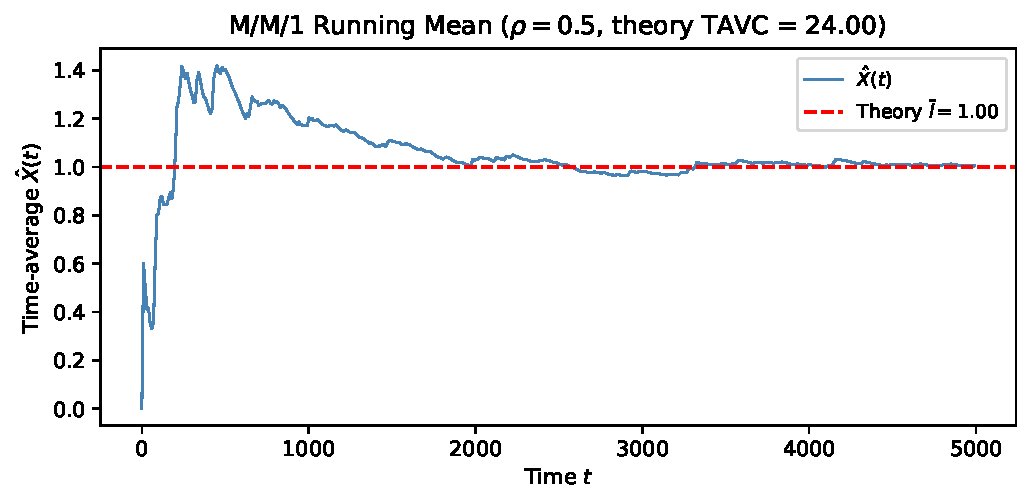
\includegraphics[width=0.50\textwidth]{tavc_illustration}
\end{center}

\framebreak

\begin{block}{TAVC for the On-Off Process (Equation 8.7.11 -- Kopocinski Formula)}
For the on-off process with on-times $T^{\mathrm{on}}$ and off-times
$T^{\mathrm{off}}$, Kopocinski derived:
\[
  \varsigma^2 = \frac{(\E T^{\mathrm{on}})^2 \mathrm{Var}[T^{\mathrm{off}}]
                    + (\E T^{\mathrm{off}})^2 \mathrm{Var}[T^{\mathrm{on}}]}
                    {(\E T^{\mathrm{on}} + \E T^{\mathrm{off}})^3}.
\]
For exponential on/off times $T^{\mathrm{on}}\sim\mathrm{Exp}(\lambda)$ and
$T^{\mathrm{off}}\sim\mathrm{Exp}(\mu)$: both have variance equal to the
square of their mean ($\mathrm{Var}[\mathrm{Exp}(r)] = 1/r^2$).  With
$\rho = \lambda/\mu$, this simplifies to (Equation 8.7.12):
\[
  \varsigma^2 = \frac{2\lambda\mu}{(\lambda+\mu)^3} = \frac{2\rho}{\mu(1+\rho)^3}.
\]
\end{block}

\begin{exampleblock}{Worked Example: TAVC of Exp/Exp On-Off Process}
Take $\lambda = 1/3$ (so $\E T^{\mathrm{on}} = 3$) and $\mu = 1$ (so
$\E T^{\mathrm{off}} = 1$).  Then $\rho = \lambda/\mu = 1/3$ and
$p = \lambda/(\lambda+\mu) = 1/4$ (the fraction of time \emph{off}).

The TAVC is:
\[
  \varsigma^2 = \frac{2 \cdot (1/3) \cdot 1}{(1/3 + 1)^3}
              = \frac{2/3}{(4/3)^3}
              = \frac{2/3}{64/27}
              = \frac{2 \cdot 27}{3 \cdot 64} = \frac{9}{32} \approx 0.281.
\]
For a target absolute error $b = 0.05$ at 95\% confidence ($z_{0.975} \approx 2$):
\[
  t_{\min} = \frac{z_{0.975}^2 \varsigma^2}{b^2}
           = \frac{4 \times 0.281}{0.0025} \approx 450 \text{ time units}.
\]
\end{exampleblock}

\end{frame}

\subsection{8.7.2 TAVC for Other Systems}

\begin{frame}[allowframebreaks]{8.7.2 TAVC for Other Systems}

\begin{block}{Whitt-Burman Formula (Equation 8.7.14) for Finite B\&D Processes}
Let $X(t)$ be a B\&D process on $\{0, 1, \ldots, n\}$ with birth rates
$\lambda_i > 0$ ($i=0,\ldots,n-1$) and death rates $\mu_i > 0$ ($i=1,\ldots,n$).
The stationary distribution satisfies $\pi \mathbf{Q} = \mathbf{0}$ (pi times Q
equals zero, where $\mathbf{Q}$ is the intensity matrix), giving:
\[
  \pi_i = \pi_0\,\frac{\lambda_0 \cdots \lambda_{i-1}}{\mu_1 \cdots \mu_i},
  \quad i=1,\ldots,n.
\]
For $Y(t) = f(X(t))$ with asymptotic mean $I_f = \sum_{i=0}^n f(i)\pi_i$,
the TAVC is given by the Whitt-Burman formula, attributed to D.Y.\ Burman:
\[
  \varsigma_f^2 = 2\sum_{j=0}^{n-1}\frac{1}{\lambda_j\pi_j}
                 \left[\sum_{i=0}^{j}(f(i)-I_f)\pi_i\right]^2.
\]
\end{block}

\textbf{M/M/1 Queue:}  The M/M/1 queue is a B\&D process on
$\{0,1,2,\ldots\}$ with $\lambda_i = \lambda$ and $\mu_i = \mu$ for all valid
$i$.  Using the covariance function of $L(t)$ (derived via the spectral method
by Reynolds), the TAVC of the queue length $L(t)$ is:
\[
  \varsigma_L^2 = \frac{2\rho(1+\rho)}{\mu(1-\rho)^4}, \qquad \rho=\lambda/\mu.
\]

This formula shows that $\varsigma_L^2$ grows as $(1-\rho)^{-4}$ as $\rho
\nearrow 1$, meaning near-critical queues require dramatically longer simulation
runs.

\textbf{M/M/$n$ Queue:}  For $n$ servers with $\lambda_i = \lambda$ and
$\mu_i = \min(i,n)\mu$, the stationary distribution is the \emph{Erlang-C
distribution} and the TAVC can be computed from the Whitt-Burman formula.

\begin{center}
  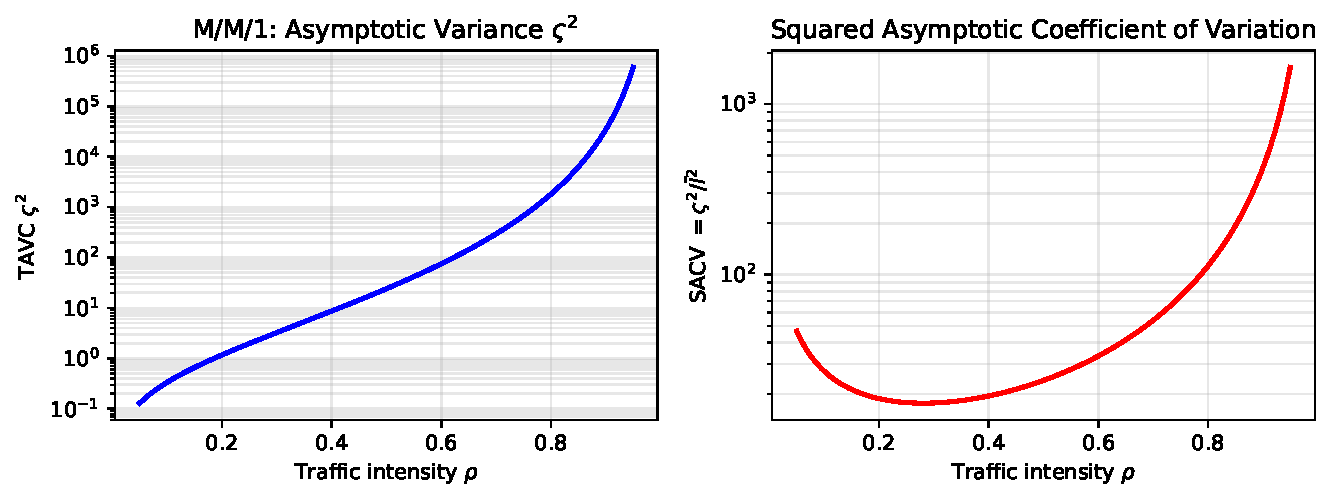
\includegraphics[width=0.55\textwidth]{tavc_vs_rho}
\end{center}

\end{frame}

% ============================================================
\section{8.8 Regenerative Processes}
% ============================================================

\begin{frame}[allowframebreaks]{8.8 Regenerative Processes}

Regenerative processes are a broad class that covers most continuous-time
queueing models.  Their key feature is that they contain random renewal times at
which the process probabilistically ``starts over'', enabling cycle-based
estimation that is often more efficient than pure time averaging.

\begin{block}{Definition 8.8.1 -- Regenerative Process}
A stochastic process $(X(t), t \ge 0)$ is \textbf{regenerative} if there exist
random times $0 = T_0 \le T_1 < T_2 < \cdots$ (regeneration times) such that
the pairs $(Z_i, C_i)_{i \ge 0}$ are independent, where:
\[
  C_0 = T_1, \quad C_i = T_{i+1} - T_i \;\; (i \ge 1)
  \qquad\text{(cycle lengths)},
\]
\[
  Z_0 = \int_0^{T_1} X(s)\,ds, \quad
  Z_i = \int_{T_i}^{T_{i+1}} X(s)\,ds \;\; (i \ge 1)
  \qquad\text{(integrals over cycles)},
\]
and $(Z_i, C_i)_{i \ge 1}$ are i.i.d.\ (identically distributed and
independent of each other).  The process \emph{restarts probabilistically}
at each $T_i$.
\end{block}

\begin{center}
  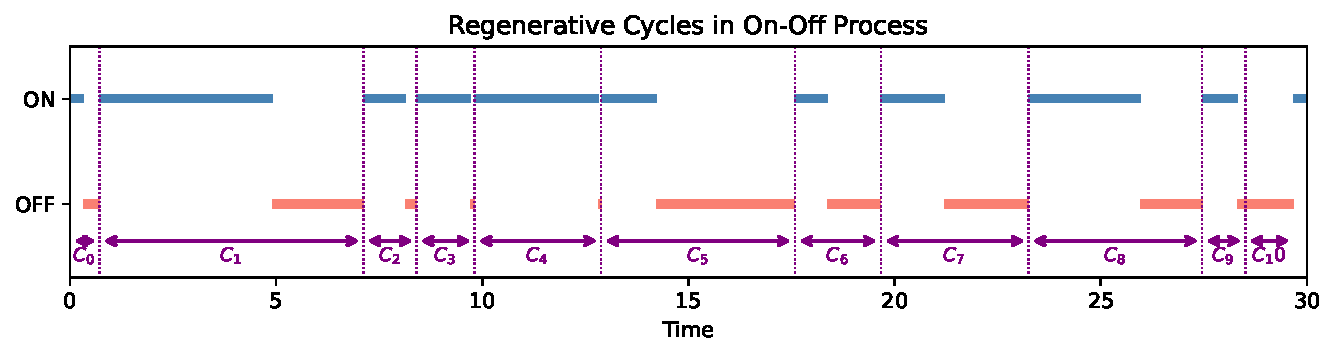
\includegraphics[width=0.74\textwidth]{regenerative_cycles}
\end{center}

\framebreak

\textbf{Examples of regenerative processes:}
\begin{itemize}
  \item \textbf{On-off process:} regenerates each time the process transitions
        to state 1 (on).  One cycle $= T^{\mathrm{on}} + T^{\mathrm{off}}$
        (one on-period plus one off-period).
  \item \textbf{M/M/1 queue:} $L(t)$ regenerates at times $T_i$ where the
        queue empties (state 0) and immediately a new arrival occurs (state 1).
        One cycle corresponds to one idle period plus one busy period.
  \item \textbf{GI/G/1 queue:} regenerates at the start of each busy period
        (when the queue goes from 0 to 1 customer).
  \item \textbf{M/G/$\infty$ queue:} regenerates when the system is empty
        and a new arrival occurs.
  \item Any irreducible positive recurrent Markov chain is regenerative with
        regeneration at return visits to any fixed state.
\end{itemize}

\begin{block}{Proposition 8.8.2 -- Renewal-Reward Theorem}
If $\E[C_1] < \infty$ and $\E[|Z_1|] < \infty$, then with probability 1
(Equation 8.8.1):
\[
  \hat{X}(t) = \frac{1}{t}\int_0^t X(s)\,ds \;\to\;
  I = \frac{\E[Z_1]}{\E[C_1]}.
\]
The steady-state mean equals the \emph{mean reward per cycle} divided by the
\emph{mean cycle length}.  If additionally $\E[C_1^2] < \infty$ and
$\mathrm{Var}[Z_1] < \infty$, a CLT holds:
\[
  \sqrt{t}(\hat{X}(t) - I) \xrightarrow{\mathcal{D}} \mathcal{N}(0,\,\varsigma_A^2),
\]
where $\varsigma_A^2 = \E[\zeta_1^2]/\E[C_1]$ and $\zeta_k = Z_k - I\,C_k$.
\end{block}

\framebreak

The renewal-reward theorem motivates a practical ratio estimator.  After
simulating $k$ complete regeneration cycles (discarding cycle 0 if the process
starts in a non-stationary state):

\begin{block}{Regenerative Ratio Estimator (Equation 8.8.6)}
\[
  \hat{I}_k = \frac{Z_1 + \cdots + Z_k}{C_1 + \cdots + C_k}.
\]
Here $Z_j$ (Z sub j) is the integral of $X(s)$ over cycle $j$, and $C_j$ (C
sub j) is the length of cycle $j$.  The ratio is the total accumulated value
divided by the total time spent in cycles.

By the law of large numbers, $\hat{I}_k \to I = \E[Z_1]/\E[C_1]$ a.s.  Under
the conditions of Proposition~8.8.2, (Proposition 8.8.6):
\[
  \sqrt{k}(\hat{I}_k - I) \xrightarrow{\mathcal{D}} \mathcal{N}(0,\,\varsigma_B^2),
  \qquad \varsigma_B^2 = \frac{\E[\zeta_1^2]}{(\E[C_1])^2}.
\]
The $1-\alpha$ confidence interval using $k$ cycles is (Equation 8.8.8):
\[
  \hat{I}_k \pm \frac{z_{1-\alpha/2}\,\hat{\varsigma}_B}{\sqrt{k}},
\]
where $\hat{\varsigma}_B^2 = \hat{\varsigma}_A^2 / \hat{C}^2$ and
$\hat{C} = \frac{1}{k}\sum_{j=1}^k C_j$ is the sample mean cycle length.
\end{block}

\textbf{Comparing $\hat{X}(t)$ vs.\ $\hat{I}_k$:}  Both have the same
asymptotic confidence interval width.  The key advantage of $\hat{X}(t)$ is
simplicity: it does not require identifying regeneration times.  The key
advantage of $\hat{I}_k$ is unbiasedness (once the first cycle is discarded)
and applicability when the simulation length is measured in cycles rather than
time.

\end{frame}

\begin{frame}[allowframebreaks]{8.8 Simulation Results for On-Off Process (Example 8.8.7)}

We illustrate both estimators on the on-off process with true $p = 3/4$,
using two choices for the on/off time distributions:
\begin{itemize}
  \item \textbf{Option 1 (Exp/Exp):} $T^{\mathrm{on}}\sim\mathrm{Exp}(1/3)$,
        $T^{\mathrm{off}}\sim\mathrm{Exp}(1)$; exponential tails.
  \item \textbf{Option 2 (Par/Gamma):} $T^{\mathrm{on}}\sim\mathrm{Par}(2.5, 1.8)$
        (Pareto distribution), $T^{\mathrm{off}}\sim\mathrm{Gamma}(2, 1/2)$;
        heavier-tailed on-times.
\end{itemize}

In both cases $\E T^{\mathrm{on}} = 3$ and $\E T^{\mathrm{off}} = 1$, giving
$p = 3/(3+1) = 0.75$.  Both estimators are computed from the same simulation
run, for $t \in [0, t_{\max}]$ with $t_{\max} = 1000$.

\begin{center}
\begin{tabular}{lcc}
  \toprule
  Quantity & Option 1 (Exp/Exp) & Option 2 (Par/Gamma) \\
  \midrule
  True $p$ & 0.75000 & 0.75000 \\
  Cycles used ($k$) & 257 & 263 \\
  $\hat{X}(t_{\max})$ & 0.72733 & 0.73932 \\
  $\hat{I}_k$ & 0.72472 & 0.73937 \\
  95\% CI for $\hat{X}(t)$ & $(0.656, 0.798)$ & $(0.701, 0.777)$ \\
  95\% CI for $\hat{I}_k$ & $(0.688, 0.761)$ & $(0.720, 0.759)$ \\
  \bottomrule
\end{tabular}
\end{center}

Both estimators bracket the true value $p=0.75$.  For Option 2 (Pareto/Gamma),
the confidence intervals are narrower because the Pareto distribution with
$\alpha=2.5 > 2$ has finite variance, leading to faster convergence.

\end{frame}

\begin{frame}[fragile]{Python: Regenerative Estimation for On-Off Process}
\begin{lstlisting}[style=python]
import numpy as np

def regenerative_onoff(F_on, F_off, n_cycles, rng=None):
    """Regenerative ratio estimator for on-off process.
    Cycles begin at each entry into the on state.
    First cycle is discarded for unbiasedness."""
    if rng is None:
        rng = np.random.default_rng()
    Zs, Cs = [], []
    for _ in range(n_cycles + 1):   # +1 to discard first cycle
        T_on  = F_on(rng)
        T_off = F_off(rng)
        C = T_on + T_off   # cycle length = on + off
        Z = T_on            # integral of K(t)=1 over cycle = on-length
        Zs.append(Z); Cs.append(C)
    Zs, Cs = np.array(Zs[1:]), np.array(Cs[1:])  # discard first
    I_hat = np.sum(Zs) / np.sum(Cs)              # ratio estimator
    # Estimate TAVC: zeta_j = Z_j - I_hat * C_j
    zeta  = Zs - I_hat * Cs
    C_bar = np.mean(Cs)
    s2_B  = np.var(zeta, ddof=1) / (C_bar ** 2)
    k = len(Zs)
    ci_half = 1.96 * np.sqrt(s2_B / k)
    return I_hat, ci_half

rng = np.random.default_rng(3)
I_hat, ci = regenerative_onoff(
    F_on  = lambda r: r.exponential(3.0),
    F_off = lambda r: r.exponential(1.0),
    n_cycles = 500, rng = rng)
print(f"I_hat = {I_hat:.5f}, 95% CI: ({I_hat-ci:.5f}, {I_hat+ci:.5f})")
print(f"True p = 0.75000")
\end{lstlisting}
\end{frame}

% ============================================================
\section{8.9 Error Analysis of M/M/1 and M/G/$\infty$}
% ============================================================

\begin{frame}[allowframebreaks]{8.9 Error Analysis of M/M/1 Queue}

We apply the TAVC framework to the M/M/1 queue to determine how long to
simulate for a given precision requirement.

The queue length $L(t)$ is a regenerative ergodically-stable process.  The
regeneration times are the moments when the queue empties and a new arrival
immediately occurs:
\[
  T_1 = \inf\{t > 0 : L(t^-) = 0,\, L(t) = 1\},
  \quad T_i = \inf\{t > T_{i-1} : L(t^-) = 0,\, L(t) = 1\}.
\]
Each regeneration cycle consists of one exponential idle period (duration
$\mathrm{Exp}(\lambda)$) followed by one busy period.

\begin{block}{M/M/1 Steady-State Quantities (with $\rho = \lambda/\mu < 1$)}
\begin{itemize}
  \item Steady-state mean queue length: $\bar{l} = \E[L^*] = \dfrac{\rho}{1-\rho}$.
  \item Steady-state variance: $\sigma_L^2 = \mathrm{Var}[L^*] = \dfrac{\rho}{(1-\rho)^2}$.
  \item TAVC (Equation 8.9.3): $\varsigma_L^2 = \dfrac{2\rho(1+\rho)}{\mu(1-\rho)^4}$.
\end{itemize}
\end{block}

The TAVC $\varsigma_L^2$ grows as $(1-\rho)^{-4}$ as $\rho \nearrow 1$.  This
means that in heavy traffic, the required simulation run length grows as the
fourth power of $1/(1-\rho)$.

\framebreak

The SACV (squared asymptotic coefficient of variation) is:
\[
  \mathrm{SACV} = \frac{\varsigma_L^2}{\bar{l}^2}
               = \frac{2\rho(1+\rho)/[\mu(1-\rho)^4]}{\rho^2/(1-\rho)^2}
               = \frac{2(1+\rho)}{\mu\rho(1-\rho)^2}.
\]
Setting a target relative error of 10\% ($b = 0.1\bar{l}$) at 95\% confidence
($z_{0.975}^2 \approx 4$):
\[
  t_{\max} = 4 \cdot \frac{\varsigma_L^2}{(0.1\bar{l})^2} = 400 \cdot \mathrm{SACV}.
\]

\begin{exampleblock}{Worked Example 8.9.1 (with $\mu = 1$)}
\textbf{Case (a): $\rho = 1/2$.}
$\bar{l} = 1$.
$\varsigma_L^2 = 2\cdot(1/2)\cdot(3/2)/[1\cdot(1/2)^4]
= (3/2)/(1/16) = 24$.
Required: $t_{\max} = 400 \cdot 24/1 = 9600$.
Simulation on $[0, 10^4]$ gave $\hat{l} = 0.9822$ (1.78\% error -- within 10\%).

\textbf{Case (b): $\rho = 8/9$.}
$\bar{l} = 8$.
$\varsigma_L^2 = 2(8/9)(17/9)/[1\cdot(1/9)^4] \approx 22032$.
Required: $t_{\max} = 400 \cdot 22032/64 \approx 1.377\times 10^5$.
Simulation on $[0, 10^4]$ gave $\hat{l} = 6.67$ (16.6\% error).
Since $10^4 \ll 1.377\times 10^5$, this large error is entirely expected.
\end{exampleblock}

\begin{columns}
  \column{0.52\textwidth}
  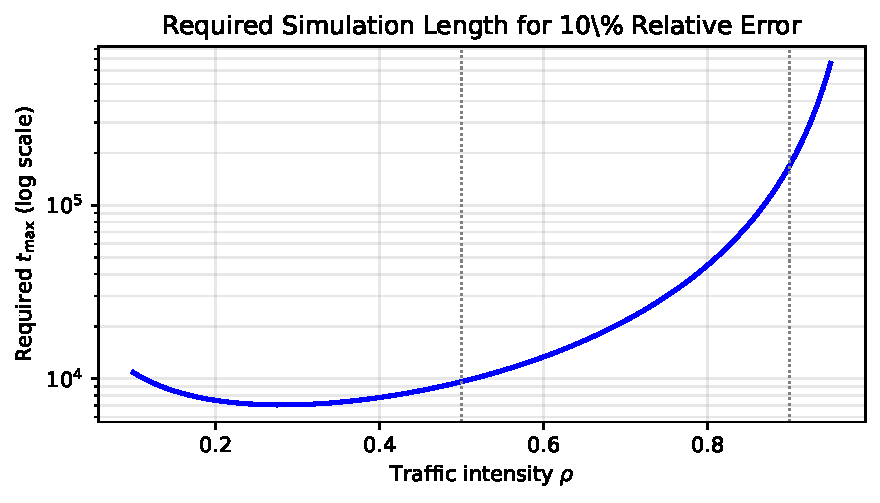
\includegraphics[width=\textwidth]{run_length_vs_rho}
  \column{0.46\textwidth}
  \textbf{Heavy traffic scaling:} As $\rho \nearrow 1$:
  \begin{itemize}
    \item For \emph{absolute} error $b$:
          $t_{\max} = O\!\left((1-\rho)^{-4}\right)$.
          From $\rho=0.5$ to $\rho=0.95$: factor $100^2 = 10\,000$ more!
    \item For \emph{relative} error:
          $t_{\max} = O\!\left((1-\rho)^{-2}\right)$.
          From $\rho=0.5$ to $\rho=0.95$: factor $100$ more.
  \end{itemize}
\end{columns}

\end{frame}

\begin{frame}[allowframebreaks]{8.9 Error Analysis of M/G/$\infty$ Systems}

For the M/G/$\infty$ queue (infinite servers, Poisson arrivals), the covariance
function can be computed explicitly from the service time distribution $G$.
This allows an exact TAVC and precise run-length requirements.

\begin{block}{M/G/$\infty$ Covariance Function and TAVC (Equation 8.9.4)}
With arrival rate $\lambda$ and service distribution $G$ with mean $\E[S]=\mu^{-1}$:
\[
  R(t) = \lambda\int_t^\infty(1-G(v))\,dv, \qquad t \ge 0.
\]
Here $G(v) = \Prob(S \le v)$ is the c.d.f.\ of the service time and
$(1-G(v))$ is the probability that service time exceeds $v$.  The TAVC is:
\[
  \varsigma^2 = 2\int_0^\infty R(t)\,dt
             = 2\lambda\int_0^\infty\int_t^\infty(1-G(v))\,dv\,dt
             = \lambda\E[S_1^2].
\]
\end{block}

This is a beautiful result: the TAVC of the M/G/$\infty$ queue equals $\lambda$
times the second moment of the service time.  For exponential service
($S \sim \mathrm{Exp}(\mu)$, $\E[S^2] = 2/\mu^2$): $\varsigma^2 = 2\lambda/\mu^2$.

\framebreak

\begin{block}{Algorithm 82 -- Simulation of M/G/$\infty$ Systems}
Each task $i$ arrives at time $A_i$ and departs at $D_i = A_i + S_i$.  The
number in the system at time $t$ is $L(t) = \sum_i \mathbf{1}(A_i \le t < D_i)$.
The integral $\int_0^{t_{\max}} L(s)\,ds$ equals
$\sum_i [\min(t_{\max}, A_i + S_i) - A_i]$
(each task $i$ contributes the portion of its sojourn that falls before $t_{\max}$).
\end{block}

The behavior depends critically on the tail of $G$.  Consider Pareto service
times $S = cX$ where $X \sim \mathrm{Par}(\alpha)$
($\Prob(X > x) = (1+x)^{-\alpha}$ for $x > 0$):
\begin{itemize}
  \item $\alpha > 3$: $\E[S^2] < \infty$, so $\varsigma^2 < \infty$ and the
        CLT holds.  The estimate converges at the normal $O(1/\sqrt{t})$ rate.
  \item $2 < \alpha \le 3$: $\E[S^2] = \infty$, $\varsigma^2 = \infty$.
        The CLT for $\hat{L}(t)$ breaks down.  A non-standard stable limit
        theorem may apply with a slower convergence rate.
  \item $1 < \alpha \le 2$: $\E[S] < \infty$ but $\E[S^2] = \infty$.  The
        estimator $\hat{L}(t)$ still converges to $\varrho$ (it is consistent),
        but extremely slowly.
\end{itemize}

\begin{columns}
  \column{0.54\textwidth}
  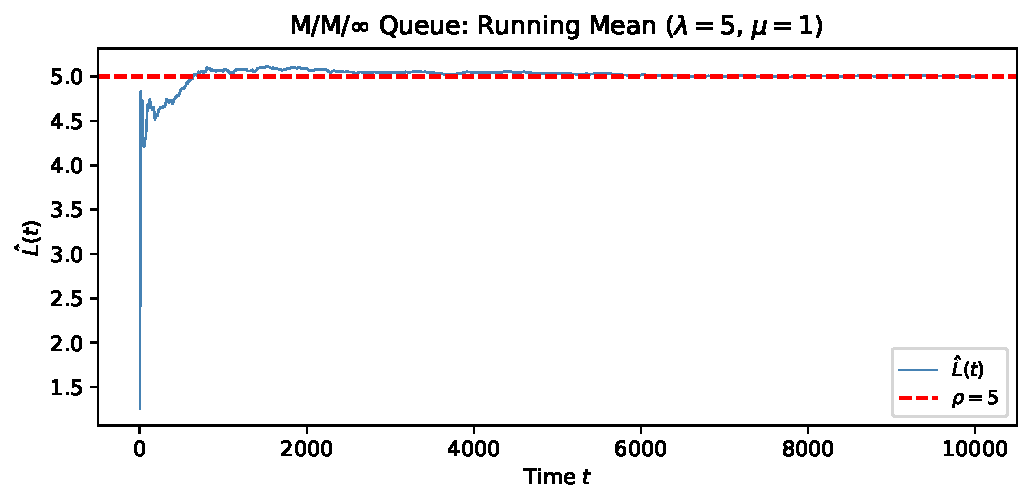
\includegraphics[width=\textwidth]{mginf_estimates}
  \column{0.44\textwidth}
  \textbf{Fig.\ 8.14:} $\hat{L}(t)$ for M/G/$\infty$ with $\lambda=5$,
  $\bar{l}=5$.\\[0.3em]
  \textbf{(a)} $S \sim \mathrm{Exp}(1)$: $\varsigma^2=10$; converges quickly.\\
  \textbf{(b)} $S=2.2X$, $X\sim\mathrm{Par}(3.2)$: $\varsigma^2=18.3$;
  needs $t > 7320$.\\
  \textbf{(c)} $S=1.2X$, $X\sim\mathrm{Par}(2.2)$: $\varsigma^2=60$;
  needs $t > 24000$.\\
  \textbf{(d)} $S=0.2X$, $X\sim\mathrm{Par}(1.2)$: $\varsigma^2=\infty$;
  CLT fails, estimate is poor ($\hat{l}=4.12$ instead of 5).
\end{columns}

\end{frame}

\begin{frame}[fragile]{Python: M/G/$\infty$ Simulation (Algorithm 82)}
\begin{lstlisting}[style=python]
import numpy as np

def simulate_mginf(lam, G_sample, t_max, rng=None):
    """Algorithm 82: Simulate M/G/inf and estimate steady-state mean.
    Uses: hat_l = sum_i [min(t_max, A_i+S_i) - A_i] / t_max"""
    if rng is None:
        rng = np.random.default_rng()
    arrivals = []
    t = rng.exponential(1.0 / lam)
    while t < t_max:
        arrivals.append(t)
        t += rng.exponential(1.0 / lam)
    arrivals = np.array(arrivals)
    if len(arrivals) == 0:
        return 0.0
    service    = G_sample(len(arrivals), rng)
    departures = arrivals + service
    # Each task contributes min(t_max, D_i) - A_i to the integral
    contribution = np.minimum(departures, t_max) - arrivals
    return np.sum(contribution) / t_max

rng = np.random.default_rng(99)
# Exponential service: theory rho=lambda/mu=5/1=5
l_hat = simulate_mginf(5.0, lambda n, r: r.exponential(1.0, n), 1e4, rng)
print(f"M/M/inf (Exp, sigma^2=10):     l_hat={l_hat:.4f} (theory=5.0)")

# Pareto(3.2) service, mean=1/(3.2-1)=0.455... scaled to mean 1
# For Par(alpha=3.2): E[S^2]=2.2^2*(1/(3.2-2)+...)
l2 = simulate_mginf(5.0, lambda n, r: r.pareto(3.2, n) * (2.2/(3.2-1)), 1e4, rng)
print(f"M/Par/inf (alpha=3.2, sigma^2=18.3): l_hat={l2:.4f} (theory=5.0)")
\end{lstlisting}
\end{frame}

% ============================================================
\section{8.10 Bibliographical Notes and Summary}
% ============================================================

\begin{frame}[allowframebreaks]{8.10 Bibliographical Notes and Algorithm Summary}

\textbf{Key references for Chapter 8:}
\begin{itemize}
  \item \textbf{Poisson processes:} Billingsley for theoretical foundations;
        classical treatment in Kingman.
  \item \textbf{Queueing theory:} Ross; Asmussen; Kleinrock (classical texts).
  \item \textbf{TAVC / SACV:} Kopocinski (on-off process formula); Whitt
        (Whitt-Burman formula for B\&D processes); Reynolds (M/M/1 covariance).
  \item \textbf{M/G/$\infty$ systems:} Rolski et al.; McNeil.
  \item \textbf{Regenerative processes:} Asmussen \& Glynn; Thorisson.
  \item \textbf{Discrete-event simulation:} Law; Bratley et al.
  \item \textbf{Random access protocols:} Bertsekas \& Gallager (ALOHA).
\end{itemize}

\vspace{0.5em}
\textbf{Summary of Chapter 8 Algorithms:}
\begin{itemize}
  \item \textbf{Alg.~73:} PoiPro($\lambda$) -- homogeneous Poisson process via
        sequential inter-arrival times.
  \item \textbf{Alg.~74:} PoiProSorted($\lambda$) -- Poisson via order statistics.
  \item \textbf{Alg.~75:} NH-Poi-thinning($\lambda(t)$) -- NHPP via thinning.
  \item \textbf{Alg.~76:} NH-Poi($\lambda(t)$) -- NHPP via inversion.
  \item \textbf{Alg.~77:} Poisson process on general space $E$.
  \item \textbf{Alg.~78:} BD -- birth-and-death process simulation.
  \item \textbf{Alg.~79:} Repairman problem -- DES with priority queue.
  \item \textbf{Algs.~80--81:} Discrete-event simulation of GI/G/c queue.
  \item \textbf{Alg.~82:} M/G/$\infty$ simulation.
\end{itemize}

\end{frame}

% ── Chapter Summary ───────────────────────────────────────
\begin{frame}[allowframebreaks]{Chapter 8 Summary}

\begin{columns}
  \column{0.50\textwidth}
  \textbf{Arrival modeling:}
  \begin{itemize}
    \item Homogeneous Poisson: inter-arrival times i.i.d.\ $\mathrm{Exp}(\lambda)$;
          simulate via sequential draws (Alg.~73) or order statistics (Alg.~74).
    \item Non-homogeneous Poisson: time-varying rate $\lambda(t)$; use thinning
          (Alg.~75) or inversion (Alg.~76).
    \item General spaces: Alg.~77 draws $K \sim \mathrm{Poi}(\Lambda(E))$
          points uniformly on $E$.
  \end{itemize}

  \textbf{Queue models:}
  \begin{itemize}
    \item M/M/1, M/M/$c$: B\&D processes; stable iff $\rho < 1$ (or $\rho < c$).
    \item GI/G/1: Lindley recursion $W_{i+1} = (W_i + S_i - \tau_{i+1})_+$.
    \item GI/G/$c$: workload vector recursion (Eq.\ 8.5.2).
    \item M/G/$\infty$: no waiting; $L^* \sim \mathrm{Poi}(\varrho)$.
    \item Slotted ALOHA: inherently unstable for any fixed $h$.
  \end{itemize}

  \column{0.48\textwidth}
  \textbf{Output analysis:}
  \begin{itemize}
    \item Time average $\hat{X}(t) \to \E[X^*]$ for ergodically stable processes.
    \item TAVC: $\varsigma^2 = 2\int_0^\infty R(v)\,dv$ (Lemma 8.7.5).
    \item Run length: $t_{\max} = z_{1-\alpha/2}^2\,\varsigma^2/b^2$.
    \item M/M/1 TAVC: $\varsigma_L^2 = 2\rho(1+\rho)/[\mu(1-\rho)^4]$.
    \item Heavy traffic: required run grows as $(1-\rho)^{-4}$ for absolute
          error, $(1-\rho)^{-2}$ for relative error.
  \end{itemize}

  \textbf{Regenerative estimation:}
  \begin{itemize}
    \item Ratio estimator $\hat{I}_k = \sum Z_j / \sum C_j$.
    \item Same asymptotic CI width as $\hat{X}(t)$.
    \item Unbiased once first cycle discarded.
    \item TAVC estimable from cycle data via $\zeta_j = Z_j - \hat{I}_k C_j$.
  \end{itemize}

  \begin{alertblock}{Central Message}
  The interplay between traffic intensity $\rho$, the TAVC $\varsigma^2$, and the
  required simulation length $t_{\max}$ governs the cost of steady-state
  simulation.  Heavy-traffic queues ($\rho \nearrow 1$) require dramatically
  longer runs to maintain the same precision.  Service time variability (via
  $\E[S^2]$) is equally important in M/G/$\infty$ and M/G/1 systems.
  \end{alertblock}
\end{columns}

\end{frame}

\end{document}
